% !TEX encoding = UTF-8
% !TEX TS-program = pdflatex
% !TEX root = ../tesi.tex

%**************************************************************
\chapter{Progettazione e codifica}
\label{cap:progettazione-codifica}
%**************************************************************

\intro{Breve introduzione al capitolo}\\
Il presente capitolo ha lo scopo di presentare e dimostrare l'architettura per i componenti IW e SP che dovranno funzionare nel contesto dell'estensione del prodotto Monokee.
%**************************************************************
\section{Componente Identity Wallet}
Questa sezione inizia con una generica introduzione all’architettura Xamarin ed infine conclude presentando una prima ipotesi di architettura in formato UML 2.0.
\subsection{Tecnologie e strumenti}
\label{sec:tecnologie-strumenti}
Il componente Identity Wallet è sviluppato come applicazione mobile, questo contesto implica differenti tecnologie che comunicano e interagiscono fra loro. Le funzionalità di persistenza vengono offerte tramite tre diverse tecnologie: file system, blockchain, e server Monokee. La logica di business è implementata usando il framework .NET. L’interfaccia, invece, usa il pattern MVVM (Model View View Model).
L’IW utilizza una classica architettura a strati (N-tier architecture). Trattandosi di un sistema mobile multi piattaforma, questa architettura è stata calata nel contesto e, quindi, si è deciso di basarla sul concetto di Portable Class Libraries (PCL) presentato da Xamarin. 

\subsubsection{Portable Class Libraries PCL}
\gls{pclg}\glsfirstoccur è un approccio alla condivisione del codice tra le diverse edizioni dell’app destinate a diversi sistemi operativi mobili sviluppato da Xamarin. Segue un diagramma esplicativo di come si sviluppa una tipica architettura PCL. Il diagramma in figura \ref{fig:ark-pcl} è tratto da \url{www.xamarin.com}.

\begin{figure}[!h]
    
    \centering
    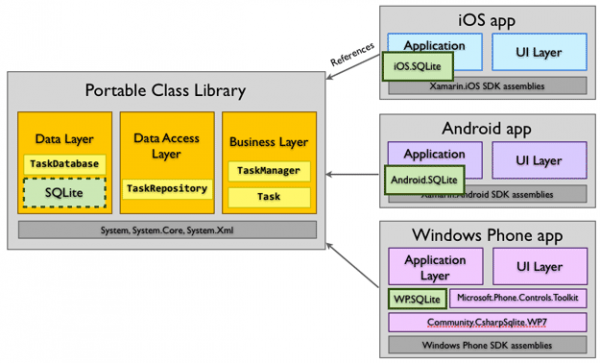
\includegraphics[width=0.9\columnwidth]{ark-pcl.png} 
    \caption{Architettura PCL}
    \label{fig:ark-pcl} 
\end{figure}

Ogni \emph{“Platform-Specific Application Project”} (iOS app, Android app, Windows Phone app) referenzia la \gls{pclg}. Quindi esistono essenzialmente due parti: quelle specifiche per la piattaforma e quelle condivise. Obiettivo del progetto è quello di rendere meno corposa possibile le parti specifiche. Sarà poi possibile impiegare caratteristiche di una determinata piattaforma attraverso l’utilizzo del design pattern \emph{Dependency Injection} (DI).
Applicare i principi della DI significa definire nel codice condiviso interfacce (classi astratte) che vengono implementate (estese) in ogni piattaforma tramite sottoclassi (\emph{Strategy Pattern}). A questo punto, sarà possibile integrare queste specifiche implementazioni all’interno della PCL. Xamarin per questo scopo offre la classe \emph{DependencyService}.


\subsection{Overview}
Come già detto l’applicativo è strutturato come una N-tier application consistente dei seguenti layer:
\begin{itemize}
    \item layer presentazione;
    \item logica di business;
    \item layer di accesso ai dati. 
\end{itemize}
    
Quando si sviluppa un’applicazione è importante scegliere se sviluppare un \emph{thin Web-based client} o \emph{un rich client}. Ovviamente, considerando il nostro contesto ricadiamo nel primo caso, infatti quasi tutta la logica e la persistenza ricadano sul componente ITF. In figura \ref{fig:ark-iw} un'immagine esplicativa dell'architettura ideata.
\begin{figure}[htbp]
    
    \centering
    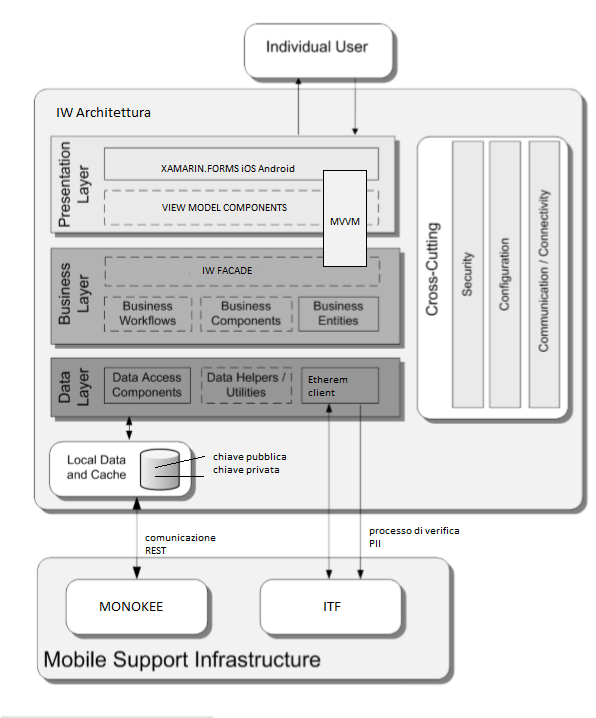
\includegraphics[width=0.9\columnwidth]{ark-iw.png} 
    \caption{Architettura PCWL}
    \label{fig:ark-iw} 
\end{figure}
Come si può notare il principale pattern utilizzato per gestire l’interazione con l’utente è il Model View ViewModel (MVVM). Tutte le elaborazioni vengono effettuate dallo strato di business, mentre per la persistenza ci si affida principalmente o alla risorsa Monokee tramite comunicazione REST, o all’ITF tramite l’utilizzo di un client Ethereum. Tutto verrà sviluppato utilizzando il framework .NET.
%**************************************************************
\subsection{Ciclo di vita del software}
\label{sec:ciclo-vita-software}

%**************************************************************
\subsection{Progettazione}
\label{sec:progettazione}
In figura \ref{fig:ark-mod-iw} viene presentato il diagramma di massima dell’architettura dell’IW. Il diagramma è stata redatto seguendo lo standard \emph{UML 2.0}. Subito a seguire viene descritta ogni classe.
\begin{figure}[htbp]
    
    \centering
    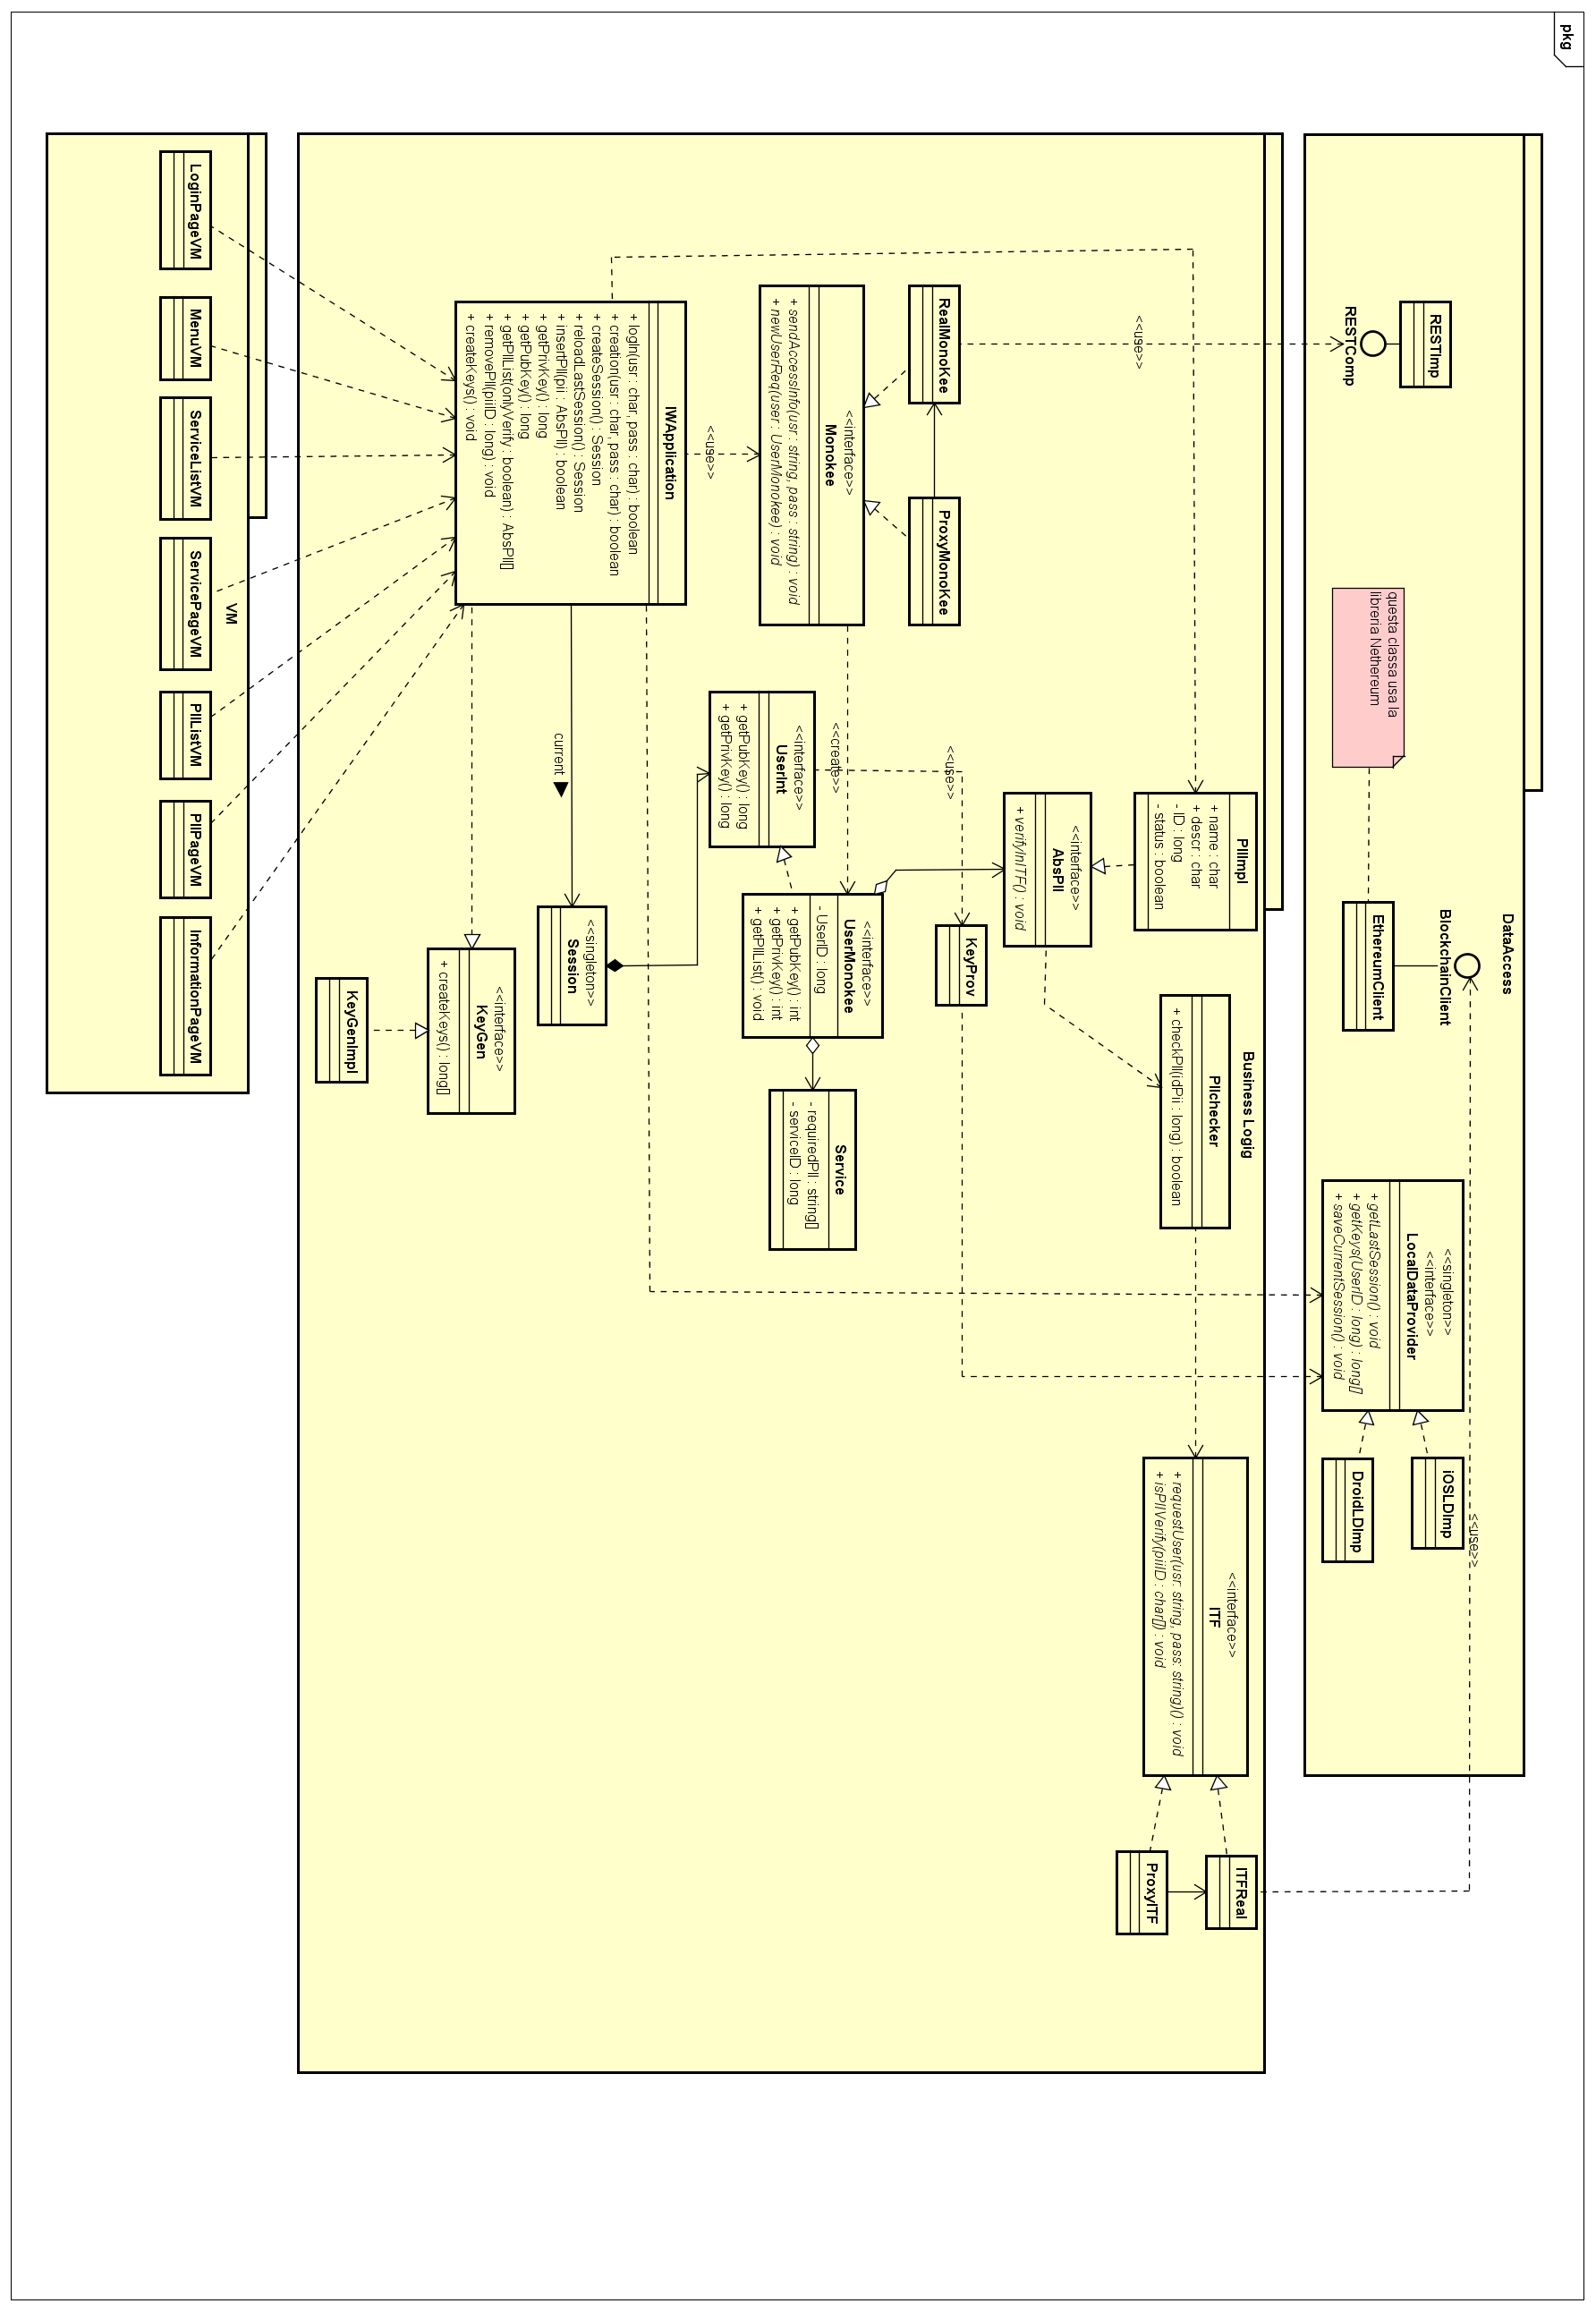
\includegraphics[width=0.9\columnwidth]{ModelArkIW.png} 
    \caption{Architettura IW}
    \label{fig:ark-mod-iw} 
\end{figure}

\paragraph{BusinessLogic} %**************************
\begin{namespacedesc}
    \classdesc{IWApplication}{questa classe ha il compito di fornire una facade per i vari ViewModel. Tutte le azioni possibile tramite l’interfaccia sono quindi implementate da questa classe.}

    \classdesc{Monokee}{ si tratta di un’interfaccia con il compito di fornire un’astrazione del servizio Monokee. Questa interfaccia con RealMonokee e ProxyMonokee rappresenta un’applicazione del pattern Proxy.}

    \classdesc{RealMonokee}{è una classe che rappresenta il reale oggetto Monokee, questa classe poi dialoga con RESTComp per ottenere i dati. Questa classe con RealMonokee e ProxyMonokee rappresenta un’applicazione del pattern Proxy.}

    \classdesc{ProxyMonokee}{è una classe che rappresenta un proxy dell’oggetto Monokee, questa classe applica una politica di acquisizione pigra. Questa classe con RealMonokee e ProxyMonokee rappresenta un’applicazione del pattern Proxy.}

    \classdesc{KeyGen}{è un’interfaccia che ha lo scopo di definire una strategia di generazione chiavi, fa parte di un’applicazione dello Strategy Pattern. È stata pensata in un’ottica in cui ci possono essere vari modi per generare una chiave a seconda del sistema operativo usato.}

    \classdesc{KeyGenImpl}{questa classe rappresenta una possibile implementazione dell’interfaccia KeyGen. Fa parte di un’applicazione dello Strategy pattern.}

    \classdesc{Session}{è una classe con lo scopo di immagazzinare tutti i dati di una sessione attiva, questa può essere generata dal file system o creata da zero. Deve essere presente in istanza singola e contiene le informazioni utente.}

    \classdesc{UserInt}{questa interfaccia rappresenta un qualsiasi utente dell’applicazione. È implementata solamente da UserMonokee. Questo oggetto viene creato dall’interfaccia Monokee.}

    \classdesc{UserMonokee}{è una classe che rappresenta un utente proveniente dal server Monokee. Implementa l’interfaccia Monokee. Un utente di questo tipo possiede un aggregato di servizi, potenzialmente contiene le chiavi e possiede una lista di PII.}

    \classdesc{Service}{è una classe che rappresenta un servizio di cui l’utente ha diritto, possiede un ID e fornisce una lista di PII che dovranno essere presentati al fine di eseguire l’accesso.}

    \classdesc{KeyProv}{è una classe che ha il compito di occuparsi della generazione delle chiavi private e pubbliche. Questa classe viene usata da UserInt e a sua volta usa LocalDataProvider.}

    \classdesc{LocalDataProvider}{è un’interfaccia che ha il compito di fornire in singolo punto dove ottenere informazione dal file system locale. Questa classe poi deve venire implementata in base al sistema operativo su cui girerà. }

    \classdesc{iOSLDImp}{ rappresenta l’implementazione per iOS di LocalDataProvider.}

    \classdesc{DroidLDImp}{rappresenta l’implementazione Android di LocalDataProvider.}

    \classdesc{AbsPII}{è un’interfaccia che rappresenta una generica PII, questa per ora ha una sola possibile implementazione, ma un’interfaccia di questo tipo renderà più semplice l’implementazione di future PII.}

    \classdesc{PIIImpl}{è una classe che rappresenta l’attuale ed unica PII. Consiste di un nome, un identificativo e una descrizione. Una PII può essere verificata o meno tramite l’uso di PIIChecker. }

    \classdesc{ITF}{si tratta di un’interfaccia con il compito di fornire un’astrazione del componente Identity Trust Fabric. Questa interfaccia con ITFReal e ProxyITF rappresenta un’applicazione del pattern Proxy.}
    \classdesc{RealITF}{è una classe che rappresenta il reale oggetto ITF, questa classe poi dialoga con il BlockchainClient per ottenere i dati. Questa classe con RealITF e ProxyITF rappresenta un’applicazione del pattern Proxy.}
    \classdesc{ProxyITF}{è una classe che rappresenta un proxy dell’oggetto Monokee, questa classe applica una politica di acquisizione pigra. Questa classe con RealITF e ProxyITF rappresenta un’applicazione del pattern Proxy.}
    \classdesc{PIIChecher}{è una classe che ha il compito di verificare tramite ITF la veridicità di una PII.}
\end{namespacedesc}

\paragraph{DataAccess} %**************************
\begin{namespacedesc}
    \classdesc{RestComp}{è un’interfaccia che ha il compito di rappresentare una generica strategia di comunicazione REST. Questa viene utilizzata da RealMonokee per ottenere i dati relativi all’utente.}
    \classdesc{RestImpl}{è una possibile implementazione della strategia di comunicazione REST. Implementa l’interfaccia RestComp.}
    \classdesc{BlockchainClient}{è un’interfaccia che ha il compito di rappresentare una generica strategia di comunicazione con la rete blockchain. Questa astrazione permette di slegare dall’architettura dipendenze con le varie implementazioni di blockchain e anche di client.}
    \classdesc{EthereumClient}{è una possibile implementazione di BlockchainClient che utilizza la rete Ethereum. Questa classe poi userà la libreria Nethereum.}
\end{namespacedesc}



\paragraph{PresentationLayer} %**************************
\begin{namespacedesc}
    \classdesc{LoginPageVM}{questa classe ha lo scopo di gestire la pagina di log in e quindi avere lo stato e le operazioni necessarie.}
    \classdesc{MenuVM}{questa classe ha lo scopo di gestire il menu dell’applicazione e quindi avere lo stato e le operazioni necessarie.}
    \classdesc{ServiceListVM}{questa classe ha lo scopo di gestire la pagina che presenta la lista dei service a cui può accedere l’utente e quindi avere lo stato e le operazioni necessarie.}
    \classdesc{ServicePage}{questa classe ha lo scopo di gestire la pagina con le informazioni relative ad un singolo servizio e quindi avere lo stato e le operazioni necessarie.}
    \classdesc{PIIListVM}{questa classe ha lo scopo di gestire la pagina che presenta la lista delle PII che possiede l’utente e quindi avere lo stato e le operazioni necessarie.}
    \classdesc{PIIPageVM}{questa classe ha lo scopo di gestire la pagina che visualizza le informazioni relative ad una specifica PII e quindi avere lo stato e le operazioni necessarie.}
    \classdesc{InformationPageVM}{questa classe ha lo scopo di gestire la pagina che fornisce le informazioni sull’applicazione, sul servizio Monokee e le istruzioni per l’uso.}
\end{namespacedesc}
%**************************************************************
\subsection{Design Pattern utilizzati}
Al fine di garantire elevate doti di qualità e manutenibilità dell’architettura sono stati usati una serie di design pattern. Di seguito segue una breve descrizione di questi.

\paragraph{Communicator}: incapsula i dettagli interni della comunicazione in un componente separato che poi può essere implementato da classi diverse e quindi canali diversi. Questo è risultato utile per rendere gli altri componenti quanto più indipendenti da come comunicano con l’esterno.

\paragraph{Data Transfer Object (DTO)}: è un oggetto che ha il compito di racchiudere le informazioni utili a diverse componenti. Questo riduce i metodi necessari per la comunicazione e in generale la semplifica.

\paragraph{Entity Translator}: Un oggetto che trasforma un dato in una forma utile per essere usato nella logica di business. Questo pattern è stato usato per interfacciarsi con il client Ethereum e il server Monokee.

\paragraph{Lazy Acquisition Proxy}: Ritarda l’acquisizione delle risorse il più a lungo possibile. Questo pattern è stato ampiamente utilizzato, specie per rendere il più leggero possibile la creazione dei dati dell’utente e della verifica dei dati nell’ITF.

\paragraph{Strategy Pattern}: è un oggetto che permette di separare l’esecuzione di un metodo dalla classe che lo contiene. Usando un’interfaccia per astrarre il metodo è poi possibile crearne molteplici implementazioni. Questo è risultato molto utile nel contesto di un’applicazione multi piattaforma in cui alcune procedure andavano implementate in nativo. Oltre all’appena citato vantaggio questo ha reso possibile separare il metodo dall’implementazione.

\paragraph{Dependency Injection}: è un pattern che permette di delegare il controllo della creazione oggetti ad un oggetto esterno. Questo permette di semplificare la gestione delle dipendenze e nel contesto dello strategy pattern permette di inoculare l’implementazione corretta.

\paragraph{Model-View-Controller}: separa il codice per l’interfaccia grafica in tre componenti separati: Modello (il dato), Vista (l’interfaccia), and Controllore (il responsabile della logica), con particolare attenzione alla vista. Nel progetto viene usata una sua particolare declinazione chiamata MVVM. 

%**************************************************************
\subsection{Progettazzione di dettaglio}
Si ricorda come l’architettura scelta in IW – Architettura di massima fosse una N-tier con tre strati. Questi sono: DataAccess Layer, BusinessLogic Layer, VMLayer. Nei prossimi capitoli verrà presentato ogni layer in maniera analitica e precisa. In figura \ref{fig:ark-dett-iw} si mostra il diagramma totale che verrà seguito durante la codifica.

\begin{figure}[htbp]
    \centering
    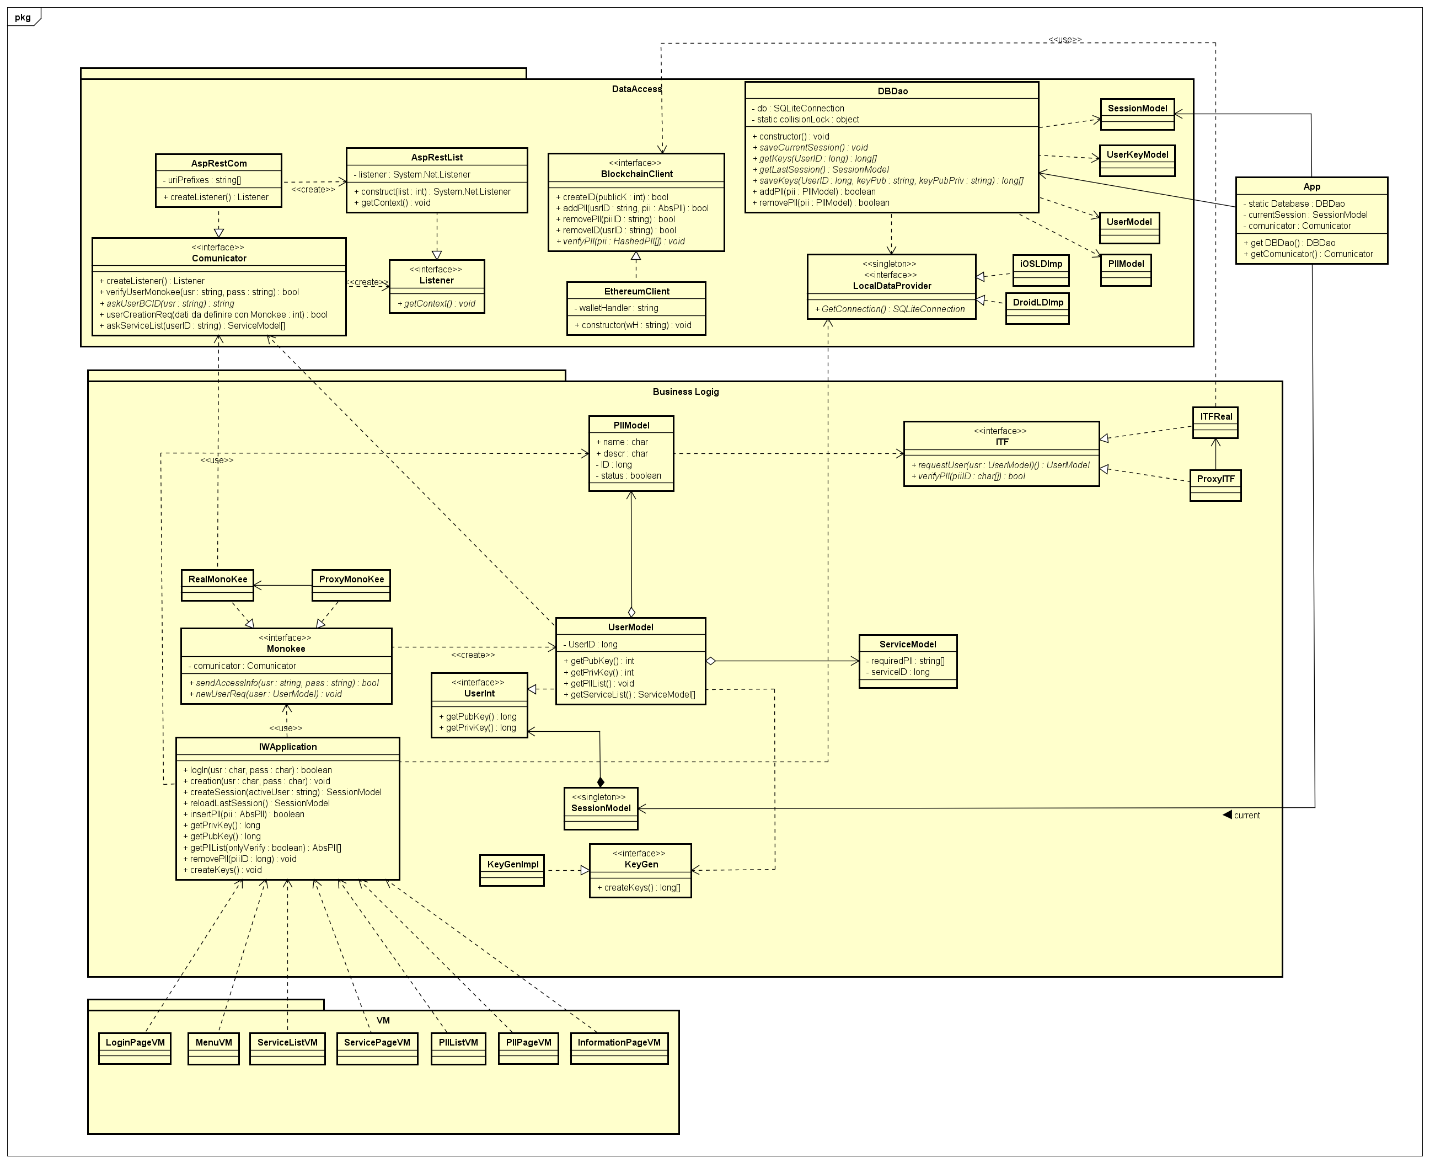
\includegraphics[width=0.9\columnwidth]{iw-complete-uml.png} 
    \caption{Architettura dettagliata IW}
    \label{fig:ark-dett-iw} 
\end{figure}
\subsubsection{DataAccess Layer}
Nel contesto dell’architettura N-tier adottata il BusinessLogic layer è un gruppo di classi che si occupano di interfacciarsi con gli strumenti di persistenza utilizzati dall’applicazione. Questi sono: Monokee (tramite RESTful), ITF e una base di dati locale al dispositivo. 
\begin{figure}[htbp]
    \centering
    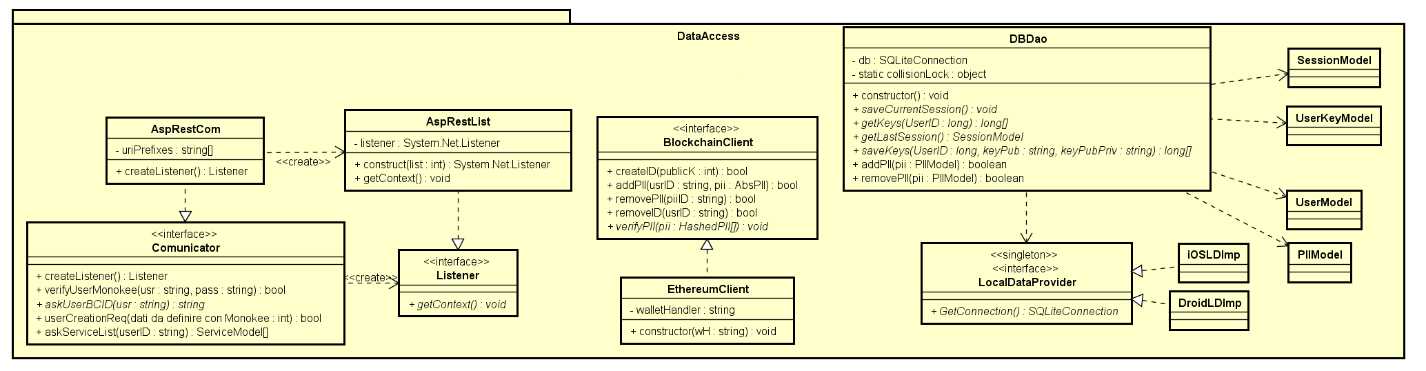
\includegraphics[width=0.9\columnwidth]{dla-iw.png} 
    \caption{Diagramma DataAccess Layer IW}
    \label{fig:dla-iw} 
\end{figure}
\paragraph{Comunicator (interfaccia)}
Questa classe fornisce un’interfaccia per gestire tutte le informazioni attraverso fonti esterne. Deve essere usata per comunicare con Monokee.
\paragraph{Metodi:}

\paragraph{Public Listener createListener()}
\begin{center}
    \begin{longtable}{|p{3cm}|p{9cm}|}%
    \caption{Public Listener createListener()}
    \label{tab:public-void-createListener}
    \endfirsthead
    \endhead
    \hline
    \textbf{Descrizione} & Il metodo ha il compito di restituire un oggetto listener che ascolto le richieste da parte di Monokee.\\
    \hline
    \textbf{Parametri} &  - \\
    \hline
    \textbf{Pseudo Codice} & Non presente \\
    \hline
    \textbf{Note} & - \\
    \hline
    \end{longtable}
    \end{center}


\paragraph{Public bool verifyUserMonokee(usr:string, pass:string)}
\begin{center}
    \begin{longtable}{|p{3cm}|p{9cm}|}%
    \caption{Public Listener createListener()}
    \label{tab:public-bool-verifyUserMonokee}
    \endfirsthead
    \endhead
    \hline
    \textbf{Descrizione} & Il metodo ha il compito di inviare una richiesta a Monokee al fine di verificare i dati forniti dall’utente. Ritorna true le l’autenticazione ha avuto successo altrimenti false.\\
    \hline
    \textbf{Parametri} &      
        \begin{itemize}
            \item usr: string che rappresenta la chiave dell’utente
            \item pass: string che rappresenta la password con cui l’utente usr tenta di effettuare l’accesso. Verificare poi come trasportare la password.
        \end{itemize}
    \\
    \hline
    \textbf{Pseudo Codice} & Non presente \\
    \hline
    \textbf{Note} & - \\
    \hline
    \end{longtable}
    \end{center}






\paragraph{Public string askUserBCID(usr:string)}
\begin{center}
    \begin{longtable}{|p{3cm}|p{9cm}|}%
    \caption{Public string askUserBCID(usr:string)}
    \label{tab:public-string-askUserBCID}
    \endfirsthead
    \endhead
    \hline
    \textbf{Descrizione} & Il metodo ha il compito di inviare una richiesta a Monokee al fine di restituire una stringa contenente l’ID sull’ITFdell’utente.\\
    \hline
    \textbf{Parametri} &      
        \begin{itemize}
            \item usr: string che rappresenta la chiave dell’utente
        \end{itemize}
    \\
    \hline
    \textbf{Pseudo Codice} & Non presente \\
    \hline
    \textbf{Note} & - \\
    \hline
    \end{longtable}
    \end{center}



\paragraph{Public bool userCreationRequest(usr: userModel)}
\begin{center}
    \begin{longtable}{|p{3cm}|p{9cm}|}%
    \caption{Public bool userCreationRequest(usr: userModel)}
    \label{tab:public-bool-userCreationRequest}
    \endfirsthead
    \endhead
    \hline
    \textbf{Descrizione} & Il metodo ha il compito di inviare una richiesta a Monokee al fine creare un utente all’interno del servizio Monokee. Questo metodo invia solo la richiesta e non ha modo di sapere il reale inserimento dell’utente. L’operazione in Monokee non è immediata.\\
    \hline
    \textbf{Parametri} &      
        \begin{itemize}
            \item usr: riferimento ad un oggetto UserModel che contiene i dati che l'utente vuole creare.
        \end{itemize}
    \\
    \hline
    \textbf{Pseudo Codice} & Non presente \\
    \hline
    \textbf{Note} & Non bisogna dare per scontato che la richiesta riceva esito positivo o che venga eseguita in maniera immediata. \\
    \hline
    \end{longtable}
    \end{center}



\paragraph{Public ServiceModel[] getServiceList(usrID:string)}
\begin{center}
    \begin{longtable}{|p{3cm}|p{9cm}|}%
    \caption{Public ServiceModel[] getServiceList(usrID:string)}
    \label{tab:public-ServiceModel[]-getServiceList}
    \endfirsthead
    \endhead
    \hline
    \textbf{Descrizione} & Il metodo ha il compito ritornare la lista dei servizi associati all’utente indicato in Monokee.  \\
    \hline
    \textbf{Parametri} &      
        \begin{itemize}
            \item usrID: stringa che rappresenta la chiave dell’utente in Monokee.
        \end{itemize}
    \\
    \hline
    \textbf{Pseudo Codice} & 
            Var com = App.getComunicator();\newline
            Return serList = await com.askServiceList(this.id);
    \\
    \hline
    \textbf{Note} & Questa informazione deve essere richiesta ogni volta, in quanto l’unico gestore di utenti e servizi e Monokee. \\
    \hline
    \end{longtable}
    \end{center}

\paragraph{AspRestCom (implementa Comunicator)}
\paragraph{Campi dati:}
\begin{itemize}
    \item \textbf{uriPrefixes}: lista stringhe che rappresentano gli uri a cui il listener ascolta. 
\end{itemize}

\paragraph{Metodi:}
\paragraph{Public Listener createListener()}
\begin{center}
    \begin{longtable}{|p{3cm}|p{9cm}|}%
    \caption{Public Listener createListener()}
    \label{tab:public-listner-createListener}
    \endfirsthead
    \endhead
    \hline
    \textbf{Descrizione} & Il metodo ha il compito di restituire un oggetto listener che ascolto le richieste da parte di Monokee.  \\
    \hline
    \textbf{Parametri} &      
        -
    \\
    \hline
    \textbf{Pseudo Codice} & 
        check (uriPrefixes not null); \newline
        check(uriPrefixes not empty) \newline
        listener = HttpListener; \newline
        foreach (uri in uriPrefixes) {
            listener.add(uri); \newline
        }
        listener.start(); \newline
        return new AspRest( listener); \newline
    \\
    \hline
    \textbf{Note} & - \\
    \hline
    \end{longtable}
    \end{center}

\paragraph{Public bool verifyUserMonokee(usr:string, pass:string)}
\begin{center}
    \begin{longtable}{|p{3cm}|p{9cm}|}%
    \caption{Public bool verifyUserMonokee(usr:string, pass:string)}
    \label{tab:public-bool-verifyUserMonokeeImpl}
    \endfirsthead
    \endhead
    \hline
    \textbf{Descrizione} & Il metodo ha il compito di inviare una richiesta a Monokee al fine di verificare i dati forniti dall’utente. Ritorna true le l’autenticazione ha avuto successo altrimenti false.  \\
    \hline
    \textbf{Parametri} &      
        \begin{itemize}
            \item usr: long che rappresenta la chiave dell’utente
            \item pass: string che rappresenta la password con cui l’utente usr tenta di effettuare l’accesso. Verificare poi come trasportare la password.
        \end{itemize}
    \\
    \hline
    \textbf{Pseudo Codice} & 
    string content =” accessReq”+usr+pass; \newline
    ASCIIEncoding encoding=new ASCIIEncoding(); \newline
    byte[]  buffer =encoding.GetBytes(content); \newline
    request.ContentType="application/x-www-IWAccessRequest "; \newline
    request.ContentLength=content.Length; \newline
    Stream newStream=request.GetRequestStream(); \newline
    newStream.Write(buffer,0,buffer.Length); \newline
    newStream.Close();
    \\
    \hline
    \textbf{Note} & \url{http://www.dotnethell.it/tips/SendPOSTHttp.aspx} \\
    \hline
    \end{longtable}
    \end{center}


    \paragraph{Public string askUserBCID(usr:string)}
    \begin{center}
        \begin{longtable}{|p{3cm}|p{9cm}|}%
        \caption{Public string askUserBCID(usr:string)}
        \label{tab:public-string-askUserBCIDImpl}
        \endfirsthead
        \endhead
        \hline
        \textbf{Descrizione} & Il metodo ha il compito di inviare una richiesta a Monokee al fine di restituire una stringa contenente l’ID sull’ITF dell’utente. \\
        \hline
        \textbf{Parametri} &      
            \begin{itemize}
                \item usr: string che rappresenta la chiave dell’utente
            \end{itemize}
        \\
        \hline
        \textbf{Pseudo Codice} & 
        string content =”ITF ID request”+usr;\newline
        ASCIIEncoding encoding=new ASCIIEncoding();\newline
        byte[]  buffer =encoding.GetBytes(content);\newline
        request.ContentType="application/x-www-ITFIDrequest ";\newline.
        request.ContentLength=content.Length;\newline
        Stream newStream=request.GetRequestStream();\newline
        newStream.Write(buffer,0,buffer.Length);\newline
        newStream.Close();\newline
        if (response != no pass) return response;\newline
        else return null;\newline
        \\
        \hline
        \textbf{Note} & \url{http://www.dotnethell.it/tips/SendPOSTHttp.aspx} \\
        \hline
        \end{longtable}
        \end{center}


    \paragraph{Public bool userCreationRequest(usr: userModel)}
    \begin{center}
        \begin{longtable}{|p{3cm}|p{9cm}|}%
        \caption{Public bool userCreationRequest(usr: userModel)}
        \label{tab:public-boll-userCreationRequestImpl}
        \endfirsthead
        \endhead
        \hline
        \textbf{Descrizione} & Il metodo ha il compito di inviare una richiesta a Monokee al fine creare un utente all’interno del servizio Monokee. Questo metodo invia solo la richiesta e non ha modo di sapere il reale inserimento dell’utente. L’operazione in Monokee non è immediata. \\
        \hline
        \textbf{Parametri} &      
            \begin{itemize}
                \item usr: riferimento ad un oggetto UserModel che contiene i dati che l'utente vuole creare.
            \end{itemize}
        \\
        \hline
        \textbf{Pseudo Codice} & 
        string content =”Monokee user creation request”+usr;\newline
        ASCIIEncoding encoding=new ASCIIEncoding();\newline
        byte[]  buffer =encoding.GetBytes(content);\newline
        request.ContentType="application/x-www-MONK-creationReq ";\newline.
        request.ContentLength=content.Length;\newline
        Stream newStream=request.GetRequestStream();\newline
        newStream.Write(buffer,0,buffer.Length);\newline
        newStream.Close();\newline
        if (response != no pass) return response;\newline
        else return null;\newline
        \\
        \hline
        \textbf{Note} & Non bisogna dare per scontato che la richiesta riceva esito positivo o che venga eseguita in maniera immediata. \\
        \hline
        \end{longtable}
        \end{center}

\paragraph{Listener (interfaccia)}
È un oggetto con il compito di rimanere in ascolto su determinati uri. È un oggetto non mutabile.
\paragraph{Metodi:}
\paragraph{Public void getContext()}
    \begin{center}
        \begin{longtable}{|p{3cm}|p{9cm}|}%
        \caption{Public void getContext()}
        \label{tab:public-void-getContext}
        \endfirsthead
        \endhead
        \hline
        \textbf{Descrizione} & Il metodo ha il compito di ritornare appena arriva un messaggio inviato da uno degli uri specificati nella AspRestComp. \\
        \hline
        \textbf{Parametri} &      
            -
        \\
        \hline
        \textbf{Pseudo Codice} & 
         Non presente \\
        \hline
        \textbf{Note} & - \\
        \hline
        \end{longtable}
        \end{center}


\paragraph{AspRestList (implementa Listerner)}
È un oggetto con il compito di rimanere in ascolto su determinati uri. È un oggetto non mutabile. Questa classe rappresenta un wrapper del listener di \emph{System.Net}.
\paragraph{Campi dati:}
\begin{itemize}
    \item listener: è il listener fornito dal System.Net. Creato da AspRestComp
\end{itemize}

\paragraph{Metodi:}
\paragraph{Public constructor()}
    \begin{center}
        \begin{longtable}{|p{3cm}|p{9cm}|}%
        \caption{Public constructor()}
        \label{tab:public-list-constructor}
        \endfirsthead
        \endhead
        \hline
        \textbf{Descrizione} & Il metodo ha il compito di costruire l’oggetto Listener da un’istanza del listener fornito da System.Net \\
        \hline
        \textbf{Parametri} &      
            \begin{itemize}
                \item List: è un’implementazione di System.Net listener.
            \end{itemize}
        \\
        \hline
        \textbf{Pseudo Codice} & 
            This.listener = List; \\
        \hline
        \textbf{Note} & - \\
        \hline
        \end{longtable}
        \end{center}


\paragraph{Public void getContext()}
\begin{center}
    \begin{longtable}{|p{3cm}|p{9cm}|}%
    \caption{Public void getContext()}
    \label{tab:public-void-getContextImpl}
    \endfirsthead
    \endhead
    \hline
    \textbf{Descrizione} & Il metodo ha il compito di ritornare appena arriva un messaggio inviato da uno degli uri specificati nella AspRestComp. \\
    \hline
    \textbf{Parametri} &      
     - \\
    \hline
    \textbf{Pseudo Codice} & 
    Listener.getContext();\\
    \hline
    \textbf{Note} & - \\
    \hline
    \end{longtable}
    \end{center}


\paragraph{BlockchainClient (interfaccia)}
Questa interfaccia ha il compito di rappresentare un canale di comunicazione verso gli SmartContract. Deve essere atea rispetto alla tipologia di \gls{blockchaing} usata.

\paragraph{Metodi:}
\paragraph{public bool verifyPII(pii: HashedPII[])}
\begin{center}
    \begin{longtable}{|p{3cm}|p{9cm}|}%
    \caption{public bool verifyPII(pii: HashedPII[])}
    \label{tab:public-bool-verifyPII}
    \endfirsthead
    \endhead
    \hline
    \textbf{Descrizione} & Il metodo ha il compito di chiamare il metodo presente negli smartContract che verifica i dati. \\
    \hline
    \textbf{Parametri} &      
    \begin{itemize}
        \item pii: è una lista di oggetti hashedPII da verificare nell’ITF.
    \end{itemize} 
    \\
    \hline
    \textbf{Pseudo Codice} & 
    Non presente\\
    \hline
    \textbf{Note} & L’implementazione sarà sensibilmente diversa in base alla specifica blockchain usata. \\
    \hline
    \end{longtable}
    \end{center}

\paragraph{public bool createID(publicK : long)}
\begin{center}
    \begin{longtable}{|p{3cm}|p{9cm}|}%
    \caption{public bool createID(publicK : long)}
    \label{tab:public-bool-createID}
    \endfirsthead
    \endhead
    \hline
    \textbf{Descrizione} & Il metodo ha il compito di chiamare il metodo presente negli smartContract che inserisce un utente nell’ITF. \\
    \hline
    \textbf{Parametri} &      
    \begin{itemize}
        \item publicK: è un long che rappresenta la chiave pubblica dell’utente creato. La chiave privata deve rimanere solo in locale nell’IW.
    \end{itemize} 
    \\
    \hline
    \textbf{Pseudo Codice} & 
    Non presente\\
    \hline
    \textbf{Note} & L’implementazione sarà sensibilmente diversa in base alla specifica blockchain usata. \\
    \hline
    \end{longtable}
    \end{center}

\paragraph{public bool addPII(usrID:string, pii:AbsPII)}
\begin{center}
    \begin{longtable}{|p{3cm}|p{9cm}|}%
    \caption{public bool addPII(usrID:string, pii:AbsPII)}
    \label{tab:public-bool-addPII}
    \endfirsthead
    \endhead
    \hline
    \textbf{Descrizione} & Il metodo ha il compito di chiamare il metodo presente negli smartContract che inserisce una nuova PII ad un utente.\\
    \hline
    \textbf{Parametri} &      
    \begin{itemize}
        \item usrID: è una stringa che rappresenta la chiave pubblica dell’utente a cui si vuole creare.
        \item Pii: è una lista di oggetti AbsPII che si vuole aggiungere all’utente identificato dalla chiave.
    \end{itemize} 
    \\
    \hline
    \textbf{Pseudo Codice} & 
    Non presente\\
    \hline
    \textbf{Note} & L’implementazione sarà sensibilmente diversa in base alla specifica blockchain usata. \\
    \hline
    \end{longtable}
    \end{center}


\paragraph{public bool removePII(piiID:string)}
\begin{center}
    \begin{longtable}{|p{3cm}|p{9cm}|}%
    \caption{public bool removePII(piiID:string)}
    \label{tab:public-bool-removePII}
    \endfirsthead
    \endhead
    \hline
    \textbf{Descrizione} & Il metodo ha il compito di chiamare il metodo presente negli smartContract che elimina una determinata PII ad un utente.\\
    \hline
    \textbf{Parametri} &      
    \begin{itemize}
        \item piiID: è una stringa che rappresenta la chiave della PII che si vuole elimare.
    \end{itemize} 
    \\
    \hline
    \textbf{Pseudo Codice} & 
    Non presente\\
    \hline
    \textbf{Note} & L’implementazione sarà sensibilmente diversa in base alla specifica blockchain usata. \\
    \hline
    \end{longtable}
    \end{center}

\paragraph{public bool removeID(usrID:string)}
\begin{center}
    \begin{longtable}{|p{3cm}|p{9cm}|}%
    \caption{public bool removeID(usrID:string)}
    \label{tab:public-bool-removeID}
    \endfirsthead
    \endhead
    \hline
    \textbf{Descrizione} & Il metodo ha il compito di chiamare il metodo presente negli smartContract che elimina un determinato utente.\\
    \hline
    \textbf{Parametri} &      
    \begin{itemize}
        \item usrID: è una stringa che rappresenta la chiave dell’utente che si vuole eliminare.
    \end{itemize} 
    \\
    \hline
    \textbf{Pseudo Codice} & 
    Non presente\\
    \hline
    \textbf{Note} & L’implementazione sarà sensibilmente diversa in base alla specifica blockchain usata. \\
    \hline
    \end{longtable}
    \end{center}
    
\paragraph{NethereumClient (implementa BlockchainClient)}
Questa classe rappresentare un canale di comunicazione verso gli \gls{SmartContractg} di una rete Ethereum. Fa uso della libreria .NET Nethereum per instaurare la comunicazione. 
\paragraph{Campi dati}
\begin{itemize}
    \item walletHandler: è una stringa che rappresenta l’indirizzo del contratto WalletHandler all’interno della blockchain. 
\end{itemize}
\paragraph{Metodi:}


\paragraph{public constructor(walletHandler: string)}
\begin{center}
    \begin{longtable}{|p{3cm}|p{9cm}|}%
    \caption{public constructor(walletHandler: string)}
    \label{tab:public-nethclient-constructor}
    \endfirsthead
    \endhead
    \hline
    \textbf{Descrizione} & Il metodo ha il compito di costruire l’oggetto Ethereum client.\\
    \hline
    \textbf{Parametri} &      
    \begin{itemize}
        \item walletHandler: è una stringa che rappresenta l’indirizzo del contratto WalletHandler.
    \end{itemize} 
    \\
    \hline
    \textbf{Pseudo Codice} & 
    This.walletHandler = walletHandler;\\
    \hline
    \textbf{Note} & - \\
    \hline
    \end{longtable}
    \end{center}


\paragraph{Public bool verifyPII(pii: HashedPII[])}
\begin{center}
    \begin{longtable}{|p{3cm}|p{9cm}|}%
    \caption{Public bool verifyPII(pii: HashedPII[])}
    \label{tab:public-bool-verifyPIIImpl}
    \endfirsthead
    \endhead
    \hline
    \textbf{Descrizione} & Il metodo ha il compito di chiamare il metodo presente negli smartContract che verifica i dati.\\
    \hline
    \textbf{Parametri} &      
    \begin{itemize}
        \item pii: è una lista di oggetti hashedPII da verificare nell’ITF.
    \end{itemize} 
    \\
    \hline
    \textbf{Pseudo Codice} & 
    Nethereum.Web3.Web3();\newline
    web3. Eth. Transactions.verifyMethod.Call;\newline
    web3. Eth. Transactions.GetTransactionReceipt;\newline
    return result;\newline
    \\
    \hline
    \textbf{Note} & \url{http://nethereum.com/} \\
    \hline
    \end{longtable}
    \end{center}

\paragraph{public bool createID(publicK : long)}
\begin{center}
    \begin{longtable}{|p{3cm}|p{9cm}|}%
    \caption{public bool createID(publicK : long)}
    \label{tab:public-bool-createIDImpl}
    \endfirsthead
    \endhead
    \hline
    \textbf{Descrizione} & Il metodo ha il compito di chiamare il metodo presente negli smartContract che inserisce un utente nell’ITF.\\
    \hline
    \textbf{Parametri} &      
    \begin{itemize}
        \item publicK: è un long che rappresenta la chiave pubblica dell’utente creato. La chiave privata deve rimanere solo in locale nell’IW.
    \end{itemize} 
    \\
    \hline
    \textbf{Pseudo Codice} & 
    Nethereum.Web3.Web3();\newline
    trova abi;\newline
    var contract = web3.Eth.GetContract(abi, walletHandler);\newline
    var createFunction = contract.GetFunction("createUser");\newline
    var result = await createFunction.CallAsync<string>(id);\newline
    \\
    \hline
    \textbf{Note} & \url{http://nethereum.com/} \\
    \hline
    \end{longtable}
    \end{center}


\paragraph{public bool createID(publicK : long)}
\begin{center}
    \begin{longtable}{|p{3cm}|p{9cm}|}%
    \caption{public bool createID(publicK : long)}
    \label{tab:public-bool-createIDImpl}
    \endfirsthead
    \endhead
    \hline
    \textbf{Descrizione} & Il metodo ha il compito di chiamare il metodo presente negli smartContract che inserisce un utente nell’ITF.\\
    \hline
    \textbf{Parametri} &      
    \begin{itemize}
        \item publicK: è un long che rappresenta la chiave pubblica dell’utente creato. La chiave privata deve rimanere solo in locale nell’IW.
    \end{itemize} 
    \\
    \hline
    \textbf{Pseudo Codice} & 
    Nethereum.Web3.Web3();\newline
    trova abi;\newline
    var contract = web3.Eth.GetContract(abi, walletHandler);\newline
    var createFunction = contract.GetFunction("createUser");\newline
    var result = await createFunction.CallAsync<string>(id);\newline
    \\
    \hline
    \textbf{Note} & \url{http://nethereum.com/} \\
    \hline
    \end{longtable}
    \end{center}


\paragraph{public bool addPII(usrID:string, pii:AbsPII)}
\begin{center}
    \begin{longtable}{|p{3cm}|p{9cm}|}%
    \caption{public bool addPII(usrID:string, pii:AbsPII)}
    \label{tab:public-bool-addPIIImpl}
    \endfirsthead
    \endhead
    \hline
    \textbf{Descrizione} & Il metodo ha il compito di chiamare il metodo presente negli smartContract che inserisce una nuova PII ad un utente.\\
    \hline
    \textbf{Parametri} &      
    \begin{itemize}
        \item usrID: è una stringa che rappresenta la chiave pubblica dell’utente a cui si vuole creare.
        \item Pii: è una lista di oggetti AbsPII che si vuole aggiungere all’utente identificato dalla chiave.
    \end{itemize} 
    \\
    \hline
    \textbf{Pseudo Codice} & 
    Nethereum.Web3.Web3();\newline
    Trova abi;\newline 
    Var contract= web3.Eth.GetContract(abi, walletHandler);\newline
    Var addPIIFunction =  contract.GetFunction(“addPII”);\newline
    Var result = await addPIIFunction.CallAsync<PII>(pii);\newline
    \\
    \hline
    \textbf{Note} & \url{http://nethereum.com/}, la chiave deve essere fornita in quanto questa verrà usata anche nel contesto dell’ITF. \\
    \hline
    \end{longtable}
    \end{center}



\paragraph{public bool removePII(piiID:string)}
\begin{center}
    \begin{longtable}{|p{3cm}|p{9cm}|}%
    \caption{public bool removePII(piiID:string)}
    \label{tab:public-bool-removePIIImpl}
    \endfirsthead
    \endhead
    \hline
    \textbf{Descrizione} & Il metodo ha il compito di chiamare il metodo presente negli smartContract che elimina una determinata PII ad un utente.\\
    \hline
    \textbf{Parametri} &      
    \begin{itemize}
        \item piiID: è una stringa che rappresenta la chiave della PII che si vuole elimare.
    \end{itemize} 
    \\
    \hline
    \textbf{Pseudo Codice} & 
    Nethereum.Web3.Web3();\newline
    trova abi(walletHandler);\newline
    var contract = web3.Eth.GetContract(abi, walletHandler);\newline
    var removeFuncition = contract.GetFunction(“removePII”);\newline
    var result = await removeFunction.CallAsync<string>(piiID);\newline
    \\
    \hline
    \textbf{Note} & \url{http://nethereum.com/}\\
    \hline
    \end{longtable}
    \end{center}

\paragraph{public bool removeID(usrID:string)}
\begin{center}
    \begin{longtable}{|p{3cm}|p{9cm}|}%
    \caption{public bool removeID(usrID:string)}
    \label{tab:public-bool-removeIDImpl}
    \endfirsthead
    \endhead
    \hline
    \textbf{Descrizione} & Il metodo ha il compito di chiamare il metodo presente negli smartContract che elimina un determinato utente.\\
    \hline
    \textbf{Parametri} &      
    \begin{itemize}
        \item usrID: è una stringa che rappresenta la chiave dell’utente che si vuole eliminare.
    \end{itemize} 
    \\
    \hline
    \textbf{Pseudo Codice} & 
    Nethereum.Web3.Web3();\newline
    trova abi(walletHandler);\newline
    var contract = web3.Eth.GetContract(abi, walletHandler);\newline
    var removeFuncition = contract.GetFunction(“removeID”);\newline
    var result = await removeFunction.CallAsync<string>(usrID);\newline
    \\
    \hline
    \textbf{Note} & \url{http://nethereum.com/}\\
    \hline
    \end{longtable}
    \end{center}

\paragraph{DBDao}
Questa classe ha il compito di fare da tramite per gli accessi al database. Rappresenta quindi il data access object relativo al database. Per effettuare la connessione viene usata la classe LocalDataProvider.
\paragraph{Campi dati:}
\begin{itemize}
    \item database: è un oggetto di tipo SQLiteConnection che rappresenta la connessione con il database
    \item static collisionLock: è un oggetto di qualsiasi tipo con lo scopo di fornire un lock all’oggetto per non permettere usi concorrenti della risorsa.
\end{itemize}

\paragraph{Metodi:}


\paragraph{public constructor()}
\begin{center}
    \begin{longtable}{|p{3cm}|p{9cm}|}%
    \caption{public constructor()}
    \label{tab:public-dao-constructor}
    \endfirsthead
    \endhead
    \hline
    \textbf{Descrizione} & Il metodo ha il compito costruire l’oggetto DBDao\\
    \hline
    \textbf{Parametri} &      
    -
    \\
    \hline
    \textbf{Pseudo Codice} & 
    database = DependencyService.Get<IRecipesDatabaseConnection>().GetConnection();\newline
    database.CreateTable<PIIModel>();\newline
    database.CreateTable<SessionModel>();\newline
    database.CreateTable<UserModel>();\newline
    \\
    \hline
    \textbf{Note} & 
    Questo metodo deve essere chiamato nella classe App del progetto nel seguente modo. 
    public static DBDao Database \newline
    { \newline
        get \newline
        { \newline
            if (database == null) \newline
            { \newline
                database = new DBDao(); \newline
            }
            return database;\newline
        }\newline
    }\newline
    Questo serve per creare l’unica istanza della base di dati all’avvio dell’applicazione.
    \\
    \hline
    \end{longtable}
    \end{center}


\paragraph{public saveCurrentSession()}
\begin{center}
    \begin{longtable}{|p{3cm}|p{9cm}|}%
    \caption{public saveCurrentSession()}
    \label{tab:public-savecurrentsession}
    \endfirsthead
    \endhead
    \hline
    \textbf{Descrizione} & Il metodo ha il compito salvare all’interno del database la sessione corrente\\
    \hline
    \textbf{Parametri} &      
    -
    \\
    \hline
    \textbf{Pseudo Codice} & 
    var sessionModel = ((IW)Application).currentSession;\newline
    lock (collisionLock)\newline
    {\newline
        if (sessionModel.Id != 0)\newline
        {\newline
            database.Update(sessionModel);\newline
            return sessionModel.Id;\newline
        }\newline
        else\newline
        {\newline
            return database.Insert(sessionModel);\newline
        }\newline
    }\newline
    \\
    \hline
    \textbf{Note} & 
    Il controllo è utile nel contesto in cui id è auto incrementale, infatti in un model creato non dal database questo viene settato a 0 di default. Anche usando gli ID provenienti dalla blockchain la cosa rimane vera in quanto non esisterebbe l’indirizzo 0.
    \\
    \hline
    \end{longtable}
    \end{center}


\paragraph{public sessionModel getLastSession()}
\begin{center}
    \begin{longtable}{|p{3cm}|p{9cm}|}%
    \caption{public sessionModel getLastSession()}
    \label{tab:public-sessionModel-getLastSession}
    \endfirsthead
    \endhead
    \hline
    \textbf{Descrizione} & Il metodo ha il compito ritornare l’ultima sessione avviata\\
    \hline
    \textbf{Parametri} &      
    -
    \\
    \hline
    \textbf{Pseudo Codice} & 
    Var last id = codice che trova il last id;\newline
    lock (collisionLock)\newline
    \{\newline
        return database.Table<sessionModel>().FirstOrDefault(x => x.Id == id);\newline
    \}\newline
    \\
    \hline
    \textbf{Note} & 
    -
    \\
    \hline
    \end{longtable}
    \end{center}


\paragraph{public UserKeyModel getKeys(userID:long)}
\begin{center}
    \begin{longtable}{|p{3cm}|p{9cm}|}%
    \caption{public UserKeyModel getKeys(userID:long)}
    \label{tab:public-userkeymodel-getKeys}
    \endfirsthead
    \endhead
    \hline
    \textbf{Descrizione} & Il metodo ha il compito ritornare la coppia di chiavi generate per l’utente specificato nel primo parametro.\\
    \hline
    \textbf{Parametri} &      
    \begin{itemize}
        \item userID: è un long che rappresenta la chiave dell’ID presente nella base di dati.
    \end{itemize}
    \\
    \hline
    \textbf{Pseudo Codice} & 
    Var last id = codice che trova il last id;\newline
    lock (collisionLock)\newline
    \{\newline
        return database.Table<sessionModel>().FirstOrDefault(x => x.Id == userID);\newline
    \}\newline
    \\
    \hline
    \textbf{Note} & 
    -
    \\
    \hline
    \end{longtable}
    \end{center}



\paragraph{Public void SaveUserKeys(usrID:string, keyPub:string, keyPriv:string)}
\begin{center}
    \begin{longtable}{|p{3cm}|p{9cm}|}%
    \caption{Public void SaveUserKeys(usrID:string, keyPub:string, keyPriv:string)}
    \label{tab:public-void-SaveUserKeys}
    \endfirsthead
    \endhead
    \hline
    \textbf{Descrizione} & Il metodo ha il compito salvare all’interno del database la sessione corrente.\\
    \hline
    \textbf{Parametri} &      
    \begin{itemize}
        \item usrID: stringa che rappresenta l’utente a cui fanno riferimento le chiavi
        \item keyPub: stringa che contiene la chiave pubblica che si vuole attribuire
        \item keyPriv: stringa che contiene la chiave privata che si vuole attribuire
    \end{itemize}
    \\
    \hline
    \textbf{Pseudo Codice} & 
    var keys = new UserKeysModel(usrID,keyPub,keyPriv);\newline
    lock (collisionLock)\newline
    \{\newline
        if (keys.userId non presente)\newline
        \{\newline
            database.Update(keys);\newline
            return keys.Id;\newline
        \}\newline
        else\newline
        \{\newline
            return database.Insert(keys);\newline
        \}\newline
    \}\newline
    \\
    \hline
    \textbf{Note} & 
    Il controllo è utile nel contesto in cui id è auto incrementale, infatti in un model creato non dal database questo viene settato a 0 di default. Anche usando gli ID provenienti dalla blockchain la cosa rimane vera in quanto non esisterebbe l’indirizzo 0.
    \\
    \hline
    \end{longtable}
    \end{center}




\paragraph{Public long addPII(pii: PIIModel)}
\begin{center}
    \begin{longtable}{|p{3cm}|p{9cm}|}%
    \caption{Public long addPII(pii: PIIModel)}
    \label{tab:public-long-addPII}
    \endfirsthead
    \endhead
    \hline
    \textbf{Descrizione} & Il metodo ha il compito salvare una PII all’interno del database. La chiave ritornata è quella decisa dall’auto incremento del database. \\
    \hline
    \textbf{Parametri} &      
    \begin{itemize}
        \item pii: è un riferimento ad un oggetto PIIModel che contiene le informazioni che si vogliono inserire all’interno della base di dati.
    \end{itemize}
    \\
    \hline
    \textbf{Pseudo Codice} & 
    lock (collisionLock)\newline
    \{\newline
        if (pii.ID non presente)\newline
        \{\newline
            database.Update(pii);\newline
            return pii.Id;\newline
        \}\newline
        else\newline
        \{\newline
            database.Insert(pii);\newline
            return pii.Id;\newline
        \} \newline
    \}\newline
    \\
    \hline
    \textbf{Note} & 
    Questa chiave identifica la PII e deve essere comunicata all’ITF.
    \\
    \hline
    \end{longtable}
    \end{center}






    \paragraph{Public long removePII(piiID: string)}
    \begin{center}
        \begin{longtable}{|p{3cm}|p{9cm}|}%
        \caption{Public long removePII(piiID: string)}
        \label{tab:public-long-removepii}
        \endfirsthead
        \endhead
        \hline
        \textbf{Descrizione} & Il metodo ha il compito rimuovere una PII all’interno del database. \\
        \hline
        \textbf{Parametri} &      
        \begin{itemize}
            \item piiID: è un riferimento ad una stringa che identifica la chiave della PII.
        \end{itemize}
        \\
        \hline
        \textbf{Pseudo Codice} & 
        lock (collisionLock)\newline
        \{\newline
            return database.Delete<PIIModel>(piiID);\newline
        \}\newline
        \\
        \hline
        \textbf{Note} & 
        La chiave è usata anche nel contesto dell’ITF.
        \\
        \hline
        \end{longtable}
        \end{center}

\paragraph{LocalDataProvider (interfaccia, singleton)}
Questa interfaccia una connessione con un database locale SQLite, Questa interfaccia deve poi essere implementata a seconda della piattaforma.
\paragraph{Metodi:}

\paragraph{public SQLiteConnection GetConnection()}
    \begin{center}
        \begin{longtable}{|p{3cm}|p{9cm}|}%
        \caption{public SQLiteConnection GetConnection()}
        \endfirsthead
        \endhead
        \hline
        \textbf{Descrizione} & Il metodo ha il compito di stabilire la connessione con il database SQLite residente nel dispositivo. Questo metodo restituisce una connessione al database.\\
        \hline
        \textbf{Parametri} &      
        -
        \\
        \hline
        \textbf{Pseudo Codice} & 
        -
        \\
        \hline
        \textbf{Note} & 
        \url{https://developer.xamarin.com/guides/android/data-and-cloud-services/data-access/part-3-using-sqlite-orm/}
        \\
        \hline
        \end{longtable}
        \end{center}

\paragraph{DroidLDImpl (implementa LocalDataProvider)}
Questa classe fornisce un’implementazione di LocalDataProvider per il sistema Android.
\paragraph{Metodi:}
        \paragraph{public SQLiteConnection GetConnection()}
        \begin{center}
            \begin{longtable}{|p{3cm}|p{9cm}|}%
            \caption{public SQLiteConnection GetConnection()}
            \endfirsthead
            \endhead
            \hline
            \textbf{Descrizione} & Il metodo ha il compito di stabilire la connessione con il database SQLite residente nel dispositivo. Questo metodo restituisce una connessione al database.\\
            \hline
            \textbf{Parametri} &      
            -
            \\
            \hline
            \textbf{Pseudo Codice} & 
            Var sqliteFilename = “RecipesDB.db3”;\newline
            String documentsPath = Environment.GetFolderPath(Environment.SpecialFolder.Personal);\newline
            String libraryPath = Path.Combine(documets,”..”,”Library”);\newline
            Var path = path.Combine(libraryPath, sqliteFilename);\newline
            Var conn = new SQLite.SQLiteConnection(path);\newline
            Return conn;\newline
            \\
            \hline
            \textbf{Note} & 
            \url{https://developer.xamarin.com/guides/android/data-and-cloud-services/data-access/part-3-using-sqlite-orm/}
            \\
            \hline
            \end{longtable}
            \end{center}
\paragraph{PIIModel (implementa INotifyPropertyChanged)}
Questa classe rappresenta un elemento della tabella nella base di dati delle PII inserite nel dispositivo.
\paragraph{Campi dati:}
\begin{itemize}
    \item name: rappresenta il nome della PII [NotNull]
    \item desc: rappresenta una string con la descrizione della PII.
    \item ID: rappresenta la chiave della PII nella base di dati e nell’ITF. [PrimaryKey, AutoIncrement] La chiave viene decisa dal database e sarà la stessa usata anche nel ITF.
    \item status: è un bool che se a true indica che la PII è stata verificata nell’ITF, se a false indica che la PII o non è stata validata.
\end{itemize}
[Table(“PIIs”)]\\
\paragraph{Metodi:}
Ogni attributo deve avere un \emph{getter} e un \emph{setter}, questi andranno implementati seguendo le funzionalità che offre C\#. Ogni setter deve chiamare \emph{PropertyChanged} al fine di garantire un corretto data binding.



\paragraph{private void PropertyChanged (propertyName)}
        \begin{center}
            \begin{longtable}{|p{3cm}|p{9cm}|}%
            \caption{private void PropertyChanged (propertyName)}
            \endfirsthead
            \endhead
            \hline
            \textbf{Descrizione} & Il metodo ha il compito di effettuare il databinding con gli oggetti che modellano la vista e il database.\\
            \hline
            \textbf{Parametri} &      
            \begin{itemize}
                \item propertyName: il nome della variabile a cui è stato effettuato il cambiamento.
            \end{itemize}
            \\
            \hline
            \textbf{Pseudo Codice} & 
            this.PropertyChanged?.Invoke(this, 
                new PropertyChangedEventArgs(propertyName));\newline
            \\
            \hline
            \textbf{Note} & 
            Questo metodo deve essere chiamato da ogni set presente nel seguente modo 
            OnPropertyChanged(nameof(nome));
            \\
            \hline
            \end{longtable}
            \end{center}

\paragraph{SessionModel (implementa INotifyPropertyChanged)}
Questa classe rappresenta un elemento della tabella nella base di dati delle Sessions inserite nel dispositivo.
\paragraph{Campi dati:}
\begin{itemize}
    \item activeUser: è un long che rappresenta la chiave all’interno del database dell’ID che ha effettuato il login nella sessione. [Foreignkey User.id]
    \item ID: rappresenta la chiave della sessione nella base di dati locale. [PrimaryKey, AutoIncrement]
\end{itemize}

In questa prima fase non sono stati definiti altri attributi, ma potrebbero essere inseriti informazioni di log quali timestamp di accesso e di log out.  

[Table(“Users”)]\\

\paragraph{Metodi:}

Ogni attributo deve avere un \emph{getter} e un \emph{setter}, questi andranno implementati seguendo le funzionalità che offre C\#. Ogni setter deve chiamare PropertyChanged al fine di garantire un corretto data binding.

\paragraph{private void PropertyChanged (propertyName)}
        \begin{center}
            \begin{longtable}{|p{3cm}|p{9cm}|}%
            \caption{private void PropertyChanged (propertyName)}
            \endfirsthead
            \endhead
            \hline
            \textbf{Descrizione} & Il metodo ha il compito di effettuare il databinding con gli oggetti che modellano la vista e il database.\\
            \hline
            \textbf{Parametri} &      
            \begin{itemize}
                \item propertyName: il nome della variabile a cui è stato effettuato il cambiamento.
            \end{itemize}
            \\
            \hline
            \textbf{Pseudo Codice} & 
            this.PropertyChanged?.Invoke(this, 
                new PropertyChangedEventArgs(propertyName));\newline
            \\
            \hline
            \textbf{Note} & 
            Questo metodo deve essere chiamato da ogni set presente nel seguente modo 
            OnPropertyChanged(nameof(nome));
            \\
            \hline
            \end{longtable}
            \end{center}


\paragraph{public void getPrivKey()}
\begin{center}
    \begin{longtable}{|p{3cm}|p{9cm}|}%
    \caption{public void getPrivKey()}
    \endfirsthead
    \endhead
    \hline
    \textbf{Descrizione} & Il metodo ha il compito ritornare la chiave privata presenta nella base di dati se presente. Se non presente genera la coppia e la ritorna.\\
    \hline
    \textbf{Parametri} &      
    \begin{itemize}
        \item propertyName: il nome della variabile a cui è stato effettuato il cambiamento.
    \end{itemize}
    \\
    \hline
    \textbf{Pseudo Codice} & 
    Var dbDao = App.getDBDao();\newline
    lock (collisionLock)\newline
        \{\newline
            Keys = dbDao.getKeys(id);\newline
        \}\newline
    If Keys == null \{\newline
        Var gen =DependencyService.Get<KeyGen>();\newline
        Long[] keys =  gen.createKeys();\newline
    dbDao.saveKeys(id, keys[0],keys[1]);\newline
    \} \newline
    return Keys[0];\newline
    \\
    \hline
    \textbf{Note} & 
    -
    \\
    \hline
    \end{longtable}
\end{center}


\paragraph{public void getPubKey()}
\begin{center}
    \begin{longtable}{|p{3cm}|p{9cm}|}%
    \caption{public void getPubKey()}
    \endfirsthead
    \endhead
    \hline
    \textbf{Descrizione} & Il metodo ha il compito ritornare la chiave pubblica presenta nella base di dati se presente. Se non presente genera la coppia e la ritorna.\\
    \hline
    \textbf{Parametri} &      
    \begin{itemize}
        \item propertyName: il nome della variabile a cui è stato effettuato il cambiamento.
    \end{itemize}
    \\
    \hline
    \textbf{Pseudo Codice} & 
    Var dbDao = App.getDBDao();\newline
    lock (collisionLock)\newline
        \{\newline
            Keys = dbDao.getKeys(id);\newline
        \}\newline
    If Keys == null \{\newline
        Var gen =DependencyService.Get<KeyGen>();\newline
        Long[] keys =  gen.createKeys();\newline
    dbDao.saveKeys(id, keys[0],keys[1]);\newline
    \} \newline
    return Keys[1];\newline
    \\
    \hline
    \textbf{Note} & 
    -
    \\
    \hline
    \end{longtable}
    \end{center}


\paragraph{Public ServiceModel[] getServiceList()}
\begin{center}
    \begin{longtable}{|p{3cm}|p{9cm}|}%
    \caption{Public ServiceModel[] getServiceList()}
    \endfirsthead
    \endhead
    \hline
    \textbf{Descrizione} & Il metodo ha il compito ritornare la lista dei servizi associati all’utente impostato come active user in Monokee.\\
    \hline
    \textbf{Parametri} &      
    -
    \\
    \hline
    \textbf{Pseudo Codice} & 
    Var com = App.getComunicator();\newline
    var id = App.currentSession.activeUser.id;\newline
    Return serList = await com.askServiceList(this.id);\newline
    \\
    \hline
    \textbf{Note} & 
    Questa informazione deve essere richiesta ogni volta, in quanto l’unico gestore di utenti e servizi e Monokee.
    \\
    \hline
    \end{longtable}
    \end{center}


\paragraph{UserKeyModel (implementa INotifyPropertyChanged)}
Questa classe rappresenta un elemento della tabella nella base di dati delle Sessions inserite nel dispositivo.
\paragraph{Campi dati:}
\begin{itemize}
    \item user: è un long che rappresenta la chiave dell’utente all’interno del database di cui fanno riferimento le informazioni. [Foreignkey User.id, PrimaryKey]
    \item KeyPriv: rappresenta la chiave pubblica. [NotNull]
    \item KeyPriv: rappresenta la chiave privata. [NotNull]
\end{itemize}
[Table(“UserKeys”)]\\
\paragraph{Metodi:}
Ogni attributo deve avere un \emph{getter} e un \emph{setter}, questi andranno implementati seguendo le funzionalità che offre C\#. Ogni setter deve chiamare PropertyChanged al fine di garantire un corretto data binding.


\paragraph{private void PropertyChanged (propertyName)}
        \begin{center}
            \begin{longtable}{|p{3cm}|p{9cm}|}%
            \caption{private void PropertyChanged (propertyName)}
            \endfirsthead
            \endhead
            \hline
            \textbf{Descrizione} & Il metodo ha il compito di effettuare il databinding con gli oggetti che modellano la vista e il database.\\
            \hline
            \textbf{Parametri} &      
            \begin{itemize}
                \item propertyName: il nome della variabile a cui è stato effettuato il cambiamento.
            \end{itemize}
            \\
            \hline
            \textbf{Pseudo Codice} & 
            this.PropertyChanged?.Invoke(this, 
                new PropertyChangedEventArgs(propertyName));\newline
            \\
            \hline
            \textbf{Note} & 
            Questo metodo deve essere chiamato da ogni set presente nel seguente modo 
            OnPropertyChanged(nameof(nome));
            \\
            \hline
            \end{longtable}
            \end{center}






\subsubsection{BusinessLogic layer}
Nel contesto dell’architettura N-tier adottata il BusinessLogic layer è un gruppo di classi che si occupano di effettuare e di mantenere tutte le regole definite dai documenti IW - Analisi di massima, IW – Studio di fattibilità.  

\begin{figure}[htbp]
    \centering
    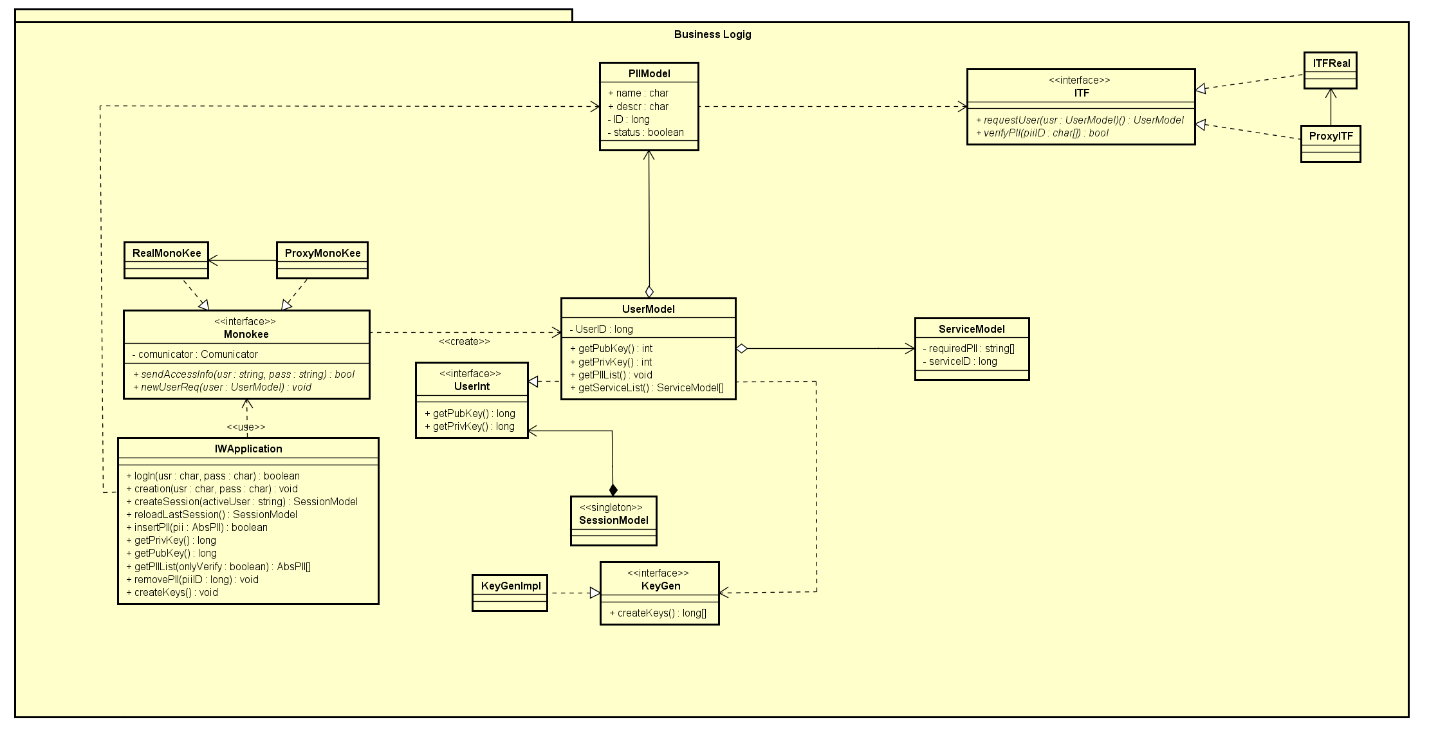
\includegraphics[width=0.9\columnwidth]{bl-lay-iw.png} 
    \caption{Diagramma BusinessLogic Layer IW}
    \label{fig:bl-lay-iw} 
\end{figure}

\paragraph{Monokee (interfaccia)}
Questa interfaccia rappresenta l’entità Monokee, con le classi RealMonokee e MonokeeProxy partecipa ad un’applicazione di un proxy pattern.

\paragraph{Metodi:}
\paragraph{Public async bool sendAccessInfo(userID: string, pass:string)}
        \begin{center}
            \begin{longtable}{|p{3cm}|p{9cm}|}%
            \caption{Public async bool sendAccessInfo(userID: string, pass:string)}
            \endfirsthead
            \endhead
            \hline
            \textbf{Descrizione} & Il metodo ha il compito di restituire true in caso i parametri passati corrispondano ad un username e una password di un utente presente nel servizio Monokee. False altrimenti. La chiamata è asincrona.\\
            \hline
            \textbf{Parametri} &      
            \begin{itemize}
                \item userID: stringa che rappresenta la chiave dell’utente
                \item pass: stringa che rappresenta la password dell’utente in chiaro.
            \end{itemize}
            \\
            \hline
            \textbf{Pseudo Codice} & 
            Non presente
            \\
            \hline
            \textbf{Note} & 
            -
            \\
            \hline
            \end{longtable}
            \end{center}




\paragraph{Public void newUserRequest(user:UserModel)}
\begin{center}
    \begin{longtable}{|p{3cm}|p{9cm}|}%
    \caption{Public void newUserRequest(user:UserModel)}
    \endfirsthead
    \endhead
    \hline
    \textbf{Descrizione} & Il metodo ha il compito di creare una richiesta di creazione utente in Monokee. Il metodo invia solo la richiesta, non ha modo di sapere se l’utente venga creato o meno.\\
    \hline
    \textbf{Parametri} &      
    \begin{itemize}
        \item user: è un riferimento ad un oggetto userModel che contiene i dati con cui si vuole inviare la richiesta di creazione l’utente.
    \end{itemize}
    \\
    \hline
    \textbf{Pseudo Codice} & 
    Non presente
    \\
    \hline
    \textbf{Note} & 
    -
    \\
    \hline
    \end{longtable}
    \end{center}



\paragraph{RealMonokee (implementa Monokee)}
Rappresenta una reale istanza del servizio Monokee. Con Monokee e MonokeeProxy rappresenta un’applicazione del pattern Proxy.
\paragraph{Campi dati:}
\begin{itemize}
    \item comunicator: è un riferimento di un oggetto che implementa l’interfaccia Comunicator.
\end{itemize}
\paragraph{Metodi:}




\paragraph{Public async bool sendAccessInfo (userID: string, pass:string)}
\begin{center}
    \begin{longtable}{|p{3cm}|p{9cm}|}%
    \caption{Public async bool sendAccessInfo (userID: string, pass:string)}
    \endfirsthead
    \endhead
    \hline
    \textbf{Descrizione} & Il metodo ha il compito di restituire true in caso i parametri passati corrispondano ad un username e una password di un utente presente nel servizio Monokee. False altrimenti.\\
    \hline
    \textbf{Parametri} &      
    \begin{itemize}
        \item userID: long che rappresenta la chiave dell’utente
        \item serviceID: long che rappresenta la chiave del servizio richiesto
    \end{itemize}
    \\
    \hline
    \textbf{Pseudo Codice} & 
    Return Async Communicator.verifyUserMonokee(userID,serviceID);
    \\
    \hline
    \textbf{Note} & 
    -
    \\
    \hline
    \end{longtable}
    \end{center}



\paragraph{Public void newUserRequest(user:UserModel)}
\begin{center}
    \begin{longtable}{|p{3cm}|p{9cm}|}%
    \caption{Public void newUserRequest(user:UserModel)}
    \endfirsthead
    \endhead
    \hline
    \textbf{Descrizione} & Il metodo ha il compito di creare una richiesta di creazione utente in Monokee. Il metodo invia solo la richiesta, non ha modo di sapere se l’utente venga creato o meno.\\
    \hline
    \textbf{Parametri} &      
    \begin{itemize}
        \item user: è un riferimento ad un oggetto userModel che contiene i dati con cui si vuole inviare la richiesta di creazione l’utente.
    \end{itemize}
    \\
    \hline
    \textbf{Pseudo Codice} & 
    Communicator.userCreationReq(user:UserModel);
    \\
    \hline
    \textbf{Note} & 
    -
    \\
    \hline
    \end{longtable}
    \end{center}


\paragraph{MonokeeProxy (implementa Monokee)}
Rappresenta un proxy remoto del servizio Monokee. Applica una politica di acquisizione pigra. Con Monokee e RealMonokee rappresenta un’applicazione del pattern Proxy.
\paragraph{Campi dati:}
\begin{itemize}
    \item realMonokee: è un riferimento di un oggetto RealMonokee.
\end{itemize}

\paragraph{Metodi:}

\paragraph{Public async bool sendAccessInfo (userID: string, pass:string)}
\begin{center}
    \begin{longtable}{|p{3cm}|p{9cm}|}%
    \caption{Public async bool sendAccessInfo (userID: string, pass:string)}
    \endfirsthead
    \endhead
    \hline
    \textbf{Descrizione} & Il metodo ha il compito di restituire true in caso i parametri passati corrispondano ad un username e una password di un utente presente nel servizio Monokee. False altrimenti.\\
    \hline
    \textbf{Parametri} &      
    \begin{itemize}
        \item userID: long che rappresenta la chiave dell’utente
        \item serviceID: long che rappresenta la chiave del servizio richiesto
    \end{itemize}
    \\
    \hline
    \textbf{Pseudo Codice} & 
    applyPolicy1;\newline
    applyPolicy2;\newline
    … \newline
    applyPolicyN;\newline
    realMonokee.sendAccessInfo(userID, pass);\newline
    \\
    \hline
    \textbf{Note} & 
    -
    \\
    \hline
    \end{longtable}
    \end{center}



\paragraph{Public void newUserRequest(user:UserModel)}
\begin{center}
    \begin{longtable}{|p{3cm}|p{9cm}|}%
    \caption{Public void newUserRequest(user:UserModel)}
    \endfirsthead
    \endhead
    \hline
    \textbf{Descrizione} & Il metodo ha il compito di creare una richiesta di creazione utente in Monokee. Il metodo invia solo la richiesta, non ha modo di sapere se l’utente venga creato o meno.\\
    \hline
    \textbf{Parametri} &      
    \begin{itemize}
        \item user: è un riferimento ad un oggetto userModel che contiene i dati con cui si vuole inviare la richiesta di creazione l’utente.
    \end{itemize}
    \\
    \hline
    \textbf{Pseudo Codice} & 
    applyPolicy1;\newline
    applyPolicy2;\newline
    …\newline
    applyPolicyN;\newline
    realMonokee.newUserRequest(user);\newline
    \\
    \hline
    \textbf{Note} & 
    -
    \\
    \hline
    \end{longtable}
    \end{center}



\paragraph{UserInt (interfaccia)}
Questa interfaccia definisce le caratteristiche minime che deve avere un utente generico dell’applicazione. Queste proprietà sono le chiavi private e pubbliche. UserModel implementa questa interfaccia. Questo ADT è stato pensato in un’ottica futura in cui ci potrebbero essere utenti non di Monokee.

\paragraph{Metodi:}
\paragraph{public void getPrivKey()}
\begin{center}
    \begin{longtable}{|p{3cm}|p{9cm}|}%
    \caption{public void getPrivKey()}
    \endfirsthead
    \endhead
    \hline
    \textbf{Descrizione} & Il metodo ha il compito ritornare la chiave privata presenta nella base di dati se presente. Se non presente genera la coppia e la ritorna.\\
    \hline
    \textbf{Parametri} &      
    -
    \\
    \hline
    \textbf{Pseudo Codice} & 
    Non presente
    \\
    \hline
    \textbf{Note} & 
    -
    \\
    \hline
    \end{longtable}
    \end{center}



\paragraph{public void getPubKey()}
\begin{center}
    \begin{longtable}{|p{3cm}|p{9cm}|}%
    \caption{public void getPubKey()}
    \endfirsthead
    \endhead
    \hline
    \textbf{Descrizione} & Il metodo ha il compito ritornare la chiave privata presenta nella base di dati se presente. Se non presente genera la coppia e la ritorna.\\
    \hline
    \textbf{Parametri} &      
    -
    \\
    \hline
    \textbf{Pseudo Codice} & 
    Non presente
    \\
    \hline
    \textbf{Note} & 
    -
    \\
    \hline
    \end{longtable}
    \end{center}

\paragraph{ServiceModel (implementa INotifyPropertyChanged)}
Questa classe rappresenta un servizio a cui l’utente può avere accesso. È definito dalla un codice e da una lista di PII richieste per effettuare l’accesso. Questo oggetto dovrà essere sempre generato da Monokee e mai salvato in locale. Questo al fine di evitare dati discordanti.
\paragraph{Campi dati:}
\begin{itemize}
    \item serviceID: è una stringa che rappresenta una chiave del servizio all’interno di Monokee.
    \item requiredPII[]: è un array di stringhe che rappresentano gli ID delle PII necessarie per effettuare il login al servizio identificato da serviceID
\end{itemize}

\paragraph{Metodi:}
Ogni attributo deve avere un \emph{getter} e un \emph{setter}, questi andranno implementati seguendo le funzionalità che offre C\#. Ogni \emph{setter} deve chiamare PropertyChanged al fine di garantire un corretto data binding.

\paragraph{private void PropertyChanged (propertyName)}
\begin{center}
    \begin{longtable}{|p{3cm}|p{9cm}|}%
    \caption{private void PropertyChanged (propertyName)}
    \endfirsthead
    \endhead
    \hline
    \textbf{Descrizione} & Il metodo ha il compito di effettuare il databinding con gli oggetti che modellano la vista e il database.\\
    \hline
    \textbf{Parametri} &      
    \begin{itemize}
        \item propertyName: il nome della variabile a cui è stato effettuato il cambiamento.
    \end{itemize}
    \\
    \hline
    \textbf{Pseudo Codice} & 
    this.PropertyChanged?.Invoke(this, 
    new PropertyChangedEventArgs(propertyName));
    \\
    \hline
    \textbf{Note} & 
    Questo metodo deve essere chiamato da ogni set presente nel seguente modo OnPropertyChanged(nameof(nome));
    \\
    \hline
    \end{longtable}
    \end{center}

\paragraph{Keygen (interfaccia)}
Questa interfaccia rappresenta un Strategy pattern per nascondere l’implementazione della reale libreria che effettua la generazione delle chiavi. Ha anche il compito di criptare e decriptare i dati.
\paragraph{Metodi:}
\paragraph{public long [] createKeys()}
\begin{center}
    \begin{longtable}{|p{3cm}|p{9cm}|}%
    \caption{public long [] createKeys()}
    \endfirsthead
    \endhead
    \hline
    \textbf{Descrizione} & Il metodo ha il compito di creare una coppia di chiavi pubbliche e private e quindi di restituirle. Ritorna un array di string di due elementi. Il primo elemento è la chiave pubblica, il secondo la privata.\\
    \hline
    \textbf{Parametri} &      
    -
    \\
    \hline
    \textbf{Pseudo Codice} & 
    Non presente.
    \\
    \hline
    \textbf{Note} & 
    -
    \\
    \hline
    \end{longtable}
    \end{center}



\paragraph{public long [] createKeys()}
\begin{center}
    \begin{longtable}{|p{3cm}|p{9cm}|}%
    \caption{public long [] createKeys()}
    \endfirsthead
    \endhead
    \hline
    \textbf{Descrizione} & Il metodo ha il compito di creare una coppia di chiavi pubbliche e private e quindi di restituirle. Ritorna un array di string di due elementi. Il primo elemento è la chiave pubblica, il secondo la privata.\\
    \hline
    \textbf{Parametri} &      
    -
    \\
    \hline
    \textbf{Pseudo Codice} & 
    Non presente.
    \\
    \hline
    \textbf{Note} & 
    -
    \\
    \hline
    \end{longtable}
    \end{center}



\paragraph{public static byte[] Encrypt(string publicKey, string data)}
\begin{center}
    \begin{longtable}{|p{3cm}|p{9cm}|}%
    \caption{public static byte[] Encrypt(string publicKey, string data)}
    \endfirsthead
    \endhead
    \hline
    \textbf{Descrizione} & Il metodo ha il compito di firmare i dati forniti con la chiave pubblica fornita.\\
    \hline
    \textbf{Parametri} &      
    \begin{itemize}
        \item publicKey: stringa che rappresenta la chiave pubblica
        \item Data: stringa che rappresenta i dati che si vogliono firmare
    \end{itemize}
    \\
    \hline
    \textbf{Pseudo Codice} & 
    Non presente.
    \\
    \hline
    \textbf{Note} & 
    -
    \\
    \hline
    \end{longtable}
    \end{center}



\paragraph{public static string Decrypt(string privateKey, byte[] encryptedBytes)}
\begin{center}
    \begin{longtable}{|p{3cm}|p{9cm}|}%
    \caption{public static string Decrypt(string privateKey, byte[] encryptedBytes)}
    \endfirsthead
    \endhead
    \hline
    \textbf{Descrizione} & Il metodo ha il compito di decriptare i dati forniti con la chiave privata fornita.\\
    \hline
    \textbf{Parametri} &      
    \begin{itemize}
        \item privateKey: stringa che rappresenta la chiave privata
        \item encryptedBytes: array di byte che rappresentano i dati che si vogliono decriptare.
    \end{itemize}
    \\
    \hline
    \textbf{Pseudo Codice} & 
    Non presente.
    \\
    \hline
    \textbf{Note} & 
    -
    \\
    \hline
    \end{longtable}
    \end{center}


\paragraph{KeygenImpl (implementa KeyGen)}
Questa interfaccia rappresenta un template pattern per nascondere l’implementazione della reale libreria che effettua la generazione delle chiavi.
\paragraph{Metodi:}

\paragraph{public static string Decrypt(string privateKey, byte[] encryptedBytes)}
\begin{center}
    \begin{longtable}{|p{3cm}|p{9cm}|}%
    \caption{public static string Decrypt(string privateKey, byte[] encryptedBytes)}
    \endfirsthead
    \endhead
    \hline
    \textbf{Descrizione} & Il metodo ha il compito di creare una coppia di chiavi pubbliche e private e quindi di restituirle. Ritorna un array di string di due elementi. Il primo elemento è la chiave pubblica, il secondo la privata.\\
    \hline
    \textbf{Parametri} &      
    -
    \\
    \hline
    \textbf{Pseudo Codice} & 
    CspParameters cspParams = new CspParameters { ProviderType = 1 };\newline

    RSACryptoServiceProvider rsaProvider = new RSACryptoServiceProvider(1024, cspParams);\newline

    string publicKey = Convert.ToBase64String(rsaProvider.ExportCspBlob(false));\newline
    string privateKey = Convert.ToBase64String(rsaProvider.ExportCspBlob(true));\newline

    return new array = {privateKey, publicKey};\newline
    \\
    \hline
    \textbf{Note} & 
    \url{https://stackoverflow.com/questions/18850030/aes-256-encryption-public-and-private-key-how-can-i-generate-and-use-it-net}
    \\
    \hline
    \end{longtable}
    \end{center}


\paragraph{public static byte[] Encrypt(string publicKey, string data)}
\begin{center}
    \begin{longtable}{|p{3cm}|p{9cm}|}%
    \caption{public static byte[] Encrypt(string publicKey, string data)}
    \endfirsthead
    \endhead
    \hline
    \textbf{Descrizione} & Il metodo ha il compito di firmare i dati forniti con la chiave pubblica fornita.\\
    \hline
    \textbf{Parametri} &      
    \begin{itemize}
        \item publicKey: stringa che rappresenta la chiave pubblica
        \item Data: stringa che rappresenta i dati che si vogliono firmare
    \end{itemize}
    \\
    \hline
    \textbf{Pseudo Codice} & 
    CspParameters cspParams = new CspParameters { ProviderType = 1 };\newline
    RSACryptoServiceProvider rsaProvider = new RSACryptoServiceProvider(cspParams);\newline
    rsaProvider.ImportCspBlob(Convert.FromBase64String(publicKey));\newline
    byte[] plainBytes = Encoding.UTF8.GetBytes(data);\newline
    byte[] encryptedBytes = rsaProvider.Encrypt(plainBytes, false);\newline
    return encryptedBytes;\newline
    \\
    \hline
    \textbf{Note} & 
    \url{https://stackoverflow.com/questions/18850030/aes-256-encryption-public-and-private-key-how-can-i-generate-and-use-it-net}
    \\
    \hline
    \end{longtable}
    \end{center}



\paragraph{public static string Decrypt(string privateKey, byte[] encryptedBytes)}
\begin{center}
    \begin{longtable}{|p{3cm}|p{9cm}|}%
    \caption{public static string Decrypt(string privateKey, byte[] encryptedBytes)}
    \endfirsthead
    \endhead
    \hline
    \textbf{Descrizione} & Il metodo ha il compito di decriptare i dati forniti con la chiave privata fornita.\\
    \hline
    \textbf{Parametri} &      
    \begin{itemize}
        \item privateKey: stringa che rappresenta la chiave privata
        \item encryptedBytes: array di byte che rappresentano i dati che si vogliono decriptare.
    \end{itemize}
    \\
    \hline
    \textbf{Pseudo Codice} & 
    CspParameters cspParams = new CspParameters { ProviderType = 1 };\item
    RSACryptoServiceProvider rsaProvider = new RSACryptoServiceProvider(cspParams);\item

    rsaProvider.ImportCspBlob(Convert.FromBase64String(privateKey));\item

    byte[] plainBytes = rsaProvider.Decrypt(encryptedBytes, false);\item

    string plainText = Encoding.UTF8.GetString(plainBytes, 0, plainBytes.Length);\item

    return plainText;\item
    \\
    \hline
    \textbf{Note} & 
    \url{https://stackoverflow.com/questions/18850030/aes-256-encryption-public-and-private-key-how-can-i-generate-and-use-it-net}
    \\
    \hline
    \end{longtable}
    \end{center}

\paragraph{ITF (interfaccia)}
Questa interfaccia rappresenta il componente ITF. Con RealITF e ITFProxy partecipano ad un’applicazione del Proxy Pattern.
\paragraph{Metodi:}


\paragraph{public verifyPII(pii: PIIModel[]):bool}
\begin{center}
    \begin{longtable}{|p{3cm}|p{9cm}|}%
    \caption{public verifyPII(pii: PIIModel[]):bool}
    \endfirsthead
    \endhead
    \hline
    \textbf{Descrizione} & Il metodo ha il compito di verificare presso l’ITF le informazioni PII. Il metodo si occupa della creazione dell’Hash.\\
    \hline
    \textbf{Parametri} &      
    \begin{itemize}
        \item pii: è una lista di oggetti PIIModel da verificare nell’ITF.
    \end{itemize}
    \\
    \hline
    \textbf{Pseudo Codice} & 
    Non presente.
    \\
    \hline
    \textbf{Note} & 
    -
    \\
    \hline
    \end{longtable}
    \end{center}



\paragraph{public requestUser(usr: userModel[]):bool}
\begin{center}
    \begin{longtable}{|p{3cm}|p{9cm}|}%
    \caption{public requestUser(usr: userModel[]):bool}
    \endfirsthead
    \endhead
    \hline
    \textbf{Descrizione} & Il metodo ha il compito creare un utente all’interno dell’ITF.\\
    \hline
    \textbf{Parametri} &      
    \begin{itemize}
        \item usr: rappresenta l’utente che si vuole immettere nell’ITF
    \end{itemize}
    \\
    \hline
    \textbf{Pseudo Codice} & 
    Non presente.
    \\
    \hline
    \textbf{Note} & 
    La chiave pubblica rappresenta l’ID dell’utente.
    \\
    \hline
    \end{longtable}
    \end{center}

\paragraph{RealITF (implementa ITF)}
Questa interfaccia rappresenta il reale componente ITF. Si occupa di instaurare la comunicazione tramite l’uso di un BlockchainClient. Con ITF e ITFProxy partecipano ad un’applicazione del Proxy Pattern.

\paragraph{Campi dati:}
tutti gli oggetti necessari vengono ottenuti tramite l’uso del DependencyService.

\paragraph{Metodi:}

\paragraph{public verifyPII(pii: PIIModel []):bool}
\begin{center}
    \begin{longtable}{|p{3cm}|p{9cm}|}%
    \caption{public verifyPII(pii: PIIModel []):bool}
    \endfirsthead
    \endhead
    \hline
    \textbf{Descrizione} & Il metodo ha il compito di verificare presso l’ITF le informazioni PII\\
    \hline
    \textbf{Parametri} &      
    \begin{itemize}
        \item pii: è una lista di oggetti hashedPII da verificare nell’ITF.
    \end{itemize}
    \\
    \hline
    \textbf{Pseudo Codice} & 
    Var blockClient = DependencyService.Get<BlockchainClient>();\newline
    HashAlgorithm algorithm = SHA256.Create();\newline
    Var hasedDesc = algorithm.ComputeHash(Encoding.UTF8.GetBytes(pii.desc));\newline
    Var hashedName = algorithm.ComputeHash(Encoding.UTF8.GetBytes(pii.name));\newline

    Return blockClient.createID(piiModel.id,hashedName, hashedDesc);\newline
    \\
    \hline
    \textbf{Note} & 
    -
    \\
    \hline
    \end{longtable}
    \end{center}



\paragraph{public bool requestUser(usr: userModel[])}
\begin{center}
    \begin{longtable}{|p{3cm}|p{9cm}|}%
    \caption{public bool requestUser(usr: userModel[])}
    \endfirsthead
    \endhead
    \hline
    \textbf{Descrizione} & Il metodo ha il compito creare un utente all’interno dell’ITF.\\
    \hline
    \textbf{Parametri} &      
    \begin{itemize}
        \item usr: rappresenta l’utente che si vuole immettere nell’ITF
    \end{itemize}
    \\
    \hline
    \textbf{Pseudo Codice} & 
    Var blockClient = DependencyService.Get<BlockchainClient>();\newline
    Return blockClient.createID(usr.getPublicKey());\newline
    \\
    \hline
    \textbf{Note} & 
    La chiave pubblica rappresenta l’ID dell’utente.
    \\
    \hline
    \end{longtable}
    \end{center}

\paragraph{ITFProxy (implementa ITF)}
Questa interfaccia rappresenta un remote proxy del componente ITF. Si occupa applicare una serie di politiche. Con ITF e ITFProxy partecipano ad un’applicazione del Proxy Pattern.
\paragraph{Campi dati:}
\begin{itemize}
    \item realITF: è un riferimento ad un oggetto RealITF. 
\end{itemize}



\paragraph{Metodi:}

\paragraph{public verifyPII(pii: PIIModel []):bool}
\begin{center}
    \begin{longtable}{|p{3cm}|p{9cm}|}%
    \caption{public verifyPII(pii: PIIModel []):bool}
    \endfirsthead
    \endhead
    \hline
    \textbf{Descrizione} & Il metodo ha il compito di verificare presso l’ITF le informazioni PII\\
    \hline
    \textbf{Parametri} &      
    \begin{itemize}
        \item pii: è una lista di oggetti hashedPII da verificare nell’ITF.
    \end{itemize}
    \\
    \hline
    \textbf{Pseudo Codice} & 
    Return realITF.verifyPII(pii);
    \\
    \hline
    \textbf{Note} & 
    -
    \\
    \hline
    \end{longtable}
    \end{center}



\paragraph{public bool requestUser(usr: userModel[])}
\begin{center}
    \begin{longtable}{|p{3cm}|p{9cm}|}%
    \caption{public bool requestUser(usr: userModel[])}
    \endfirsthead
    \endhead
    \hline
    \textbf{Descrizione} & Il metodo ha il compito creare un utente all’interno dell’ITF.\\
    \hline
    \textbf{Parametri} &      
    \begin{itemize}
        \item usr: rappresenta l’utente che si vuole immettere nell’ITF
    \end{itemize}
    \\
    \hline
    \textbf{Pseudo Codice} & 
    realITF. requestUser(usr: userModel[]);
    \\
    \hline
    \textbf{Note} & 
    La chiave pubblica rappresenta l’ID dell’utente.
    \\
    \hline
    \end{longtable}
    \end{center}

\paragraph{IWApplication}
Questa classe rappresenta un facade che espone tutte le funzioni che può compiere un utente attraverso le varie viste.
\paragraph{Campi dati:}
\begin{itemize}
    \item monokee: è un riferimento ad un oggetto che implementa l’interfaccia Monokee.
    \item database: è un riferimento ad un oggetto DBDao ottenuto tramite l’uso di DependecyService.
\end{itemize}

\paragraph{Metodi:}

\paragraph{public bool logIn(usr: string, pass:string)}
\begin{center}
    \begin{longtable}{|p{3cm}|p{9cm}|}%
    \caption{public bool logIn(usr: string, pass:string)}
    \endfirsthead
    \endhead
    \hline
    \textbf{Descrizione} & Il metodo ha il compito di verificare che le credenziali fornite dall’utente corrispondano anche nel servizio Monokee.\\
    \hline
    \textbf{Parametri} &      
    \begin{itemize}
        \item  usr: rappresenta la chiave dell’utente
        \item Pass: è una stringa che rappresenta la password dell’utente
    \end{itemize}
    \\
    \hline
    \textbf{Pseudo Codice} & 
    Var b = Monokee.sendAccessInfo(usr, pass);\newline
    Return b;\newline
    \\
    \hline
    \textbf{Note} & 
    -
    \\
    \hline
    \end{longtable}
    \end{center}


\paragraph{public void creation(usr: string, pass:string)}
\begin{center}
    \begin{longtable}{|p{3cm}|p{9cm}|}%
    \caption{public void creation(usr: string, pass:string)}
    \endfirsthead
    \endhead
    \hline
    \textbf{Descrizione} & Il metodo ha il compito di inviare una richiesta di creazione utente di un utente. Questo metodo invia solo una richiesta, non a modo di sapere se l’utente verrà effettivamente creato.\\
    \hline
    \textbf{Parametri} &      
    \begin{itemize}
        \item  usr: rappresenta la chiave dell’utente
        \item Pass: è una stringa che rappresenta la password dell’utente
    \end{itemize}
    \\
    \hline
    \textbf{Pseudo Codice} & 
    Var b = Monokee.newUserRequest(usr, pass);\newline
    Return b;\newline
    \\
    \hline
    \textbf{Note} & 
    -
    \\
    \hline
    \end{longtable}
    \end{center}


\paragraph{public void createSession(activeUser: string)}
\begin{center}
    \begin{longtable}{|p{3cm}|p{9cm}|}%
    \caption{public void createSession(activeUser: string)}
    \endfirsthead
    \endhead
    \hline
    \textbf{Descrizione} & Il metodo ha il compito creare la sessione e di inserirla nel database come lastSession.\\
    \hline
    \textbf{Parametri} &      
    \begin{itemize}
        \item  usr: rappresenta la chiave dell’utente
        \item Pass: è una stringa che rappresenta la password dell’utente
    \end{itemize}
    \\
    \hline
    \textbf{Pseudo Codice} & 
    currentSession = new SessionModel(activeUser.id);\newline
    App.currentSession = currentSession;\newline
    Database.saveCurrentSession();\newline
    \\
    \hline
    \textbf{Note} & 
    La current session è mantenuta nell’oggetto App.
    \\
    \hline
    \end{longtable}
    \end{center}



\paragraph{public void reloadLastSession()}
\begin{center}
    \begin{longtable}{|p{3cm}|p{9cm}|}%
    \caption{public void reloadLastSession()}
    \endfirsthead
    \endhead
    \hline
    \textbf{Descrizione} & Il metodo ha il compito ricaricare l’ultima sessione dal database e ritornala.\\
    \hline
    \textbf{Parametri} &      
    \begin{itemize}
        \item  usr: rappresenta la chiave dell’utente
        \item Pass: è una stringa che rappresenta la password dell’utente
    \end{itemize}
    \\
    \hline
    \textbf{Pseudo Codice} & 
    Return database.getLastSession();
    \\
    \hline
    \textbf{Note} & 
    -
    \\
    \hline
    \end{longtable}
    \end{center}



\paragraph{public void insertPII(pii:PIIModel)}
\begin{center}
    \begin{longtable}{|p{3cm}|p{9cm}|}%
    \caption{public void insertPII(pii:PIIModel)}
    \endfirsthead
    \endhead
    \hline
    \textbf{Descrizione} & Il metodo ha il compito inserire la pii all’utente corrente e anche all’interno dell’ITF.\\
    \hline
    \textbf{Parametri} &      
    \begin{itemize}
        \item pii: rappresenta la PII che si vuole inserire all’utente corrente
    \end{itemize}
    \\
    \hline
    \textbf{Pseudo Codice} & 
    Database.addPII(pii,status = false)\newline
    BlockchainClient.addPII\newline
    (App.currentSession.activeUser, pii);\newline
    \\
    \hline
    \textbf{Note} & 
    \\
    \hline
    \end{longtable}
    \end{center}

    \paragraph{public void getPrivKey()}
    \begin{center}
        \begin{longtable}{|p{3cm}|p{9cm}|}%
        \caption{public void getPrivKey()}
        \endfirsthead
        \endhead
        \hline
        \textbf{Descrizione} & Il metodo ha il compito ritornare la chiave privata dell’utente che indicato come active user nella sessione corrente.\\
        \hline
        \textbf{Parametri} &      
        \begin{itemize}
            \item pii: rappresenta la PII che si vuole inserire all’utente corrente
        \end{itemize}
        \\
        \hline
        \textbf{Pseudo Codice} & 
        Return BlockchainClient\newline
        .addPII(App.currentSession\newline
        .activeUser.getPrivKey();\newline
        \\
        \hline
        \textbf{Note} & 
        -
        \\
        \hline
        \end{longtable}
        \end{center}
    
\paragraph{public void getPubKey()}
\begin{center}
    \begin{longtable}{|p{3cm}|p{9cm}|}%
    \caption{public void getPubKey()}
    \endfirsthead
    \endhead
    \hline
    \textbf{Descrizione} & Il metodo ha il compito ritornare la chiave Pubblica dell’utente che indicato come active user nella sessione corrente.\\
    \hline
    \textbf{Parametri} &      
    \begin{itemize}
        \item pii: rappresenta la PII che si vuole inserire all’utente corrente
    \end{itemize}
    \\
    \hline
    \textbf{Pseudo Codice} & 
    Return BlockchainClient\newline
    .addPII(App.currentSession\newline
    .activeUser.getPUBKey();\newline
    \\
    \hline
    \textbf{Note} & 
    -
    \\
    \hline
    \end{longtable}
\end{center}

\paragraph{public void getPIIList()}
\begin{center}
    \begin{longtable}{|p{3cm}|p{9cm}|}%
    \caption{public void getPIIList()}
    \endfirsthead
    \endhead
    \hline
    \textbf{Descrizione} & Il metodo ha il compito ritornare la lista di PII dell’utente che è indicato come active user nella sessione corrente.\\
    \hline
    \textbf{Parametri} &      
    \begin{itemize}
        \item pii: rappresenta la PII che si vuole inserire all’utente corrente
    \end{itemize}
    \\
    \hline
    \textbf{Pseudo Codice} & 
    Return \newline
    App.currentSession \newline
    .activeUser.getPIIList(); \newline
    \\
    \hline
    \textbf{Note} & 
    -
    \\
    \hline
    \end{longtable}
\end{center}

\paragraph{public void removePII(pii:string)}
\begin{center}
    \begin{longtable}{|p{3cm}|p{9cm}|}%
    \caption{public void removePII(pii:string)}
    \endfirsthead
    \endhead
    \hline
    \textbf{Descrizione} & Il metodo ha il compito inserire la pii all’utente corrente e anche all’interno dell’ITF.\\
    \hline
    \textbf{Parametri} &      
    \begin{itemize}
        \item pii: rappresenta la chiave dellla PII che si vuole inserire all’utente corrente
    \end{itemize}
    \\
    \hline
    \textbf{Pseudo Codice} & 
    Database.removePII(pii,status = false)\newline
    BlockchainClient.removePII(pii);\newline
    \\
    \hline
    \textbf{Note} & 
    -
    \\
    \hline
    \end{longtable}
\end{center}



\paragraph{public Tuple<string,string> createKeys()}
\begin{center}
    \begin{longtable}{|p{3cm}|p{9cm}|}%
    \caption{public Tuple<string,string> createKeys()}
    \endfirsthead
    \endhead
    \hline
    \textbf{Descrizione} & Il metodo ha il compito di creare all’utente corrente un paio di chiavi asincrone.\\
    \hline
    \textbf{Parametri} &      
    \begin{itemize}
        \item pii: rappresenta la chiave dellla PII che si vuole inserire all’utente corrente
    \end{itemize}
    \\
    \hline
    \textbf{Pseudo Codice} & 
    Var a = BlockchainClient \newline
    .addPII(App.currentSession.activeUser.getPriv(); \newline
    Var b = BlockchainClient \newline
    .addPII(App.currentSession.activeUser.getPubl(); \newline
    Return new Tuple<string,string>(a,b); \newline
    \\
    \hline
    \textbf{Note} & 
    L’algoritmo usato è SHA3 per questione di compatibilità con l'ITF.
    \\
    \hline
    \end{longtable}
\end{center}

\paragraph{IQRGenerator (interfaccia)}
Questa interfaccia rappresenta uno strategy Pattern per accomunare le varie implementazioni di algoritmi che generano una lista di byte che rappresentano immagini di codici QR.
\paragraph{Metodi:}

\paragraph{public byte[] generateQR(value: string)}
\begin{center}
    \begin{longtable}{|p{3cm}|p{9cm}|}%
    \caption{public byte[] generateQR(value: string)}
    \endfirsthead
    \endhead
    \hline
    \textbf{Descrizione} & Il metodo ha il compito di creare un’array di byte che rappresentano un’immagine del codice QR contenente la stringa definita in value.\\
    \hline
    \textbf{Parametri} &      
    \begin{itemize}
        \item value: è una stringa che rappresenta il testo che si vuole inserire dentro il QR.
    \end{itemize}
    \\
    \hline
    \textbf{Pseudo Codice} & 
    Non presente
    \\
    \hline
    \textbf{Note} & 
    -
    \\
    \hline
    \end{longtable}
\end{center}

\paragraph{IQRGenerator (implementa IQRgenerator)}
Questa classe rappresenta un’implementazione dell’algoritmo di generazione QR per Android.
\paragraph{Metodi:}

\paragraph{public byte[] generateQR(value: string)}
\begin{center}
    \begin{longtable}{|p{3cm}|p{9cm}|}%
    \caption{public byte[] generateQR(value: string)}
    \endfirsthead
    \endhead
    \hline
    \textbf{Descrizione} & Il metodo ha il compito di creare un’array di byte che rappresentano un’immagine del codice QR contenente la stringa definita in value.\\
    \hline
    \textbf{Parametri} &      
    \begin{itemize}
        \item value: è una stringa che rappresenta il testo che si vuole inserire dentro il QR.
    \end{itemize}
    \\
    \hline
    \textbf{Pseudo Codice} & 
    var writer = \newline
    new BarcodeWriter \newline
    \{\newline
        Format = BarcodeFormat.QRCODE,\newline
        Options = new EncodingOptions\newline
        \{\newline
            Height = 1600,\newline
            Width = 1600\newline
        \}\newline
    \};\newline
    Android.Graphics.Bitmap bm =  writer.Write(value);\newline
    MemoryStream stream = new MemoryStream();\newline
    bm.Compress(Bitmap.CompressFormat.Jpeg, 100, stream);\newline
    var arr =  stream.ToArray();\newline
    stream.Close();\newline
    return arr;\newline
    \\
    \hline
    \textbf{Note} & 
    -
    \\
    \hline
    \end{longtable}
\end{center}


\subsubsection{VM Layer}
Questo layer contiene i vari controllori che gestiscono le viste. Si è previsto di creare un controller per ogni pagina dell’applicazione. L’applicazione utilizza il pattern MVVM, quindi, i controlli sono delle ViewModel (VM) che contengono i dati e le operazioni. Tra i dati e la vista sono presenti dei binding da realizzare utilizzando gli strumenti forniti da Xamarin. Le VM operano le loro azioni tramite l’utilizzo della classe IWFacade. 

Esiste un controllore per ogni vista prevista dall’applicazione. Le seguenti sono:
\begin{itemize}
    \item LoginPageVM;
    \item MenuVM;
    \item ServiceListVM;
    \item ServicePageVM;
    \item PIIListVM;
    \item PIIPage;
    \item AddPIIPageVM.
\end{itemize}
Tutte queste classi devono estendere da INotifyPropertyChanged.
In figura \ref{fig:vm-layer-iw} il diagramma esplicativo del \emph{layer}.

\begin{figure}[htbp]
    \centering
    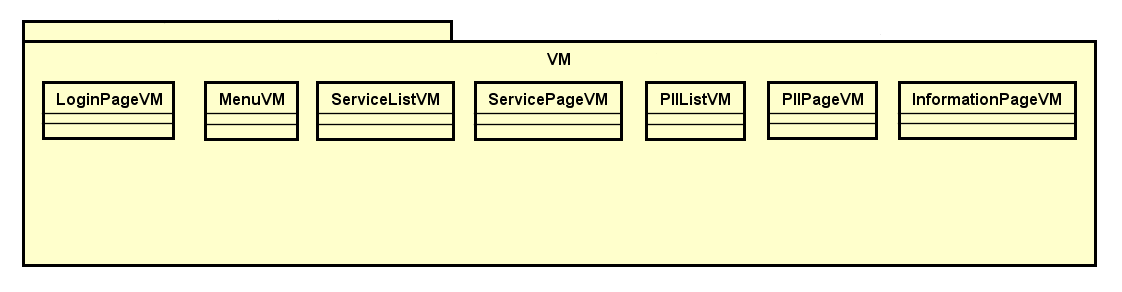
\includegraphics[width=0.9\columnwidth]{VMlayer-iw.png} 
    \caption{Diagramma UML VM Layer}
    \label{fig:vm-layer-iw} 
\end{figure}

\paragraph{LoginPageVM (implementa INotifyPropertyChanged)}
È il controllore della pagina di login.
\paragraph{Campi dati:}
\begin{itemize}
    \item DisplayInvalidLoginPrompt: è un rifermento ad un oggetto Action (Xamarin) che definisce l’azione da intaprendere in caso di credenziali errate. Questo oggetto è definito nel code-behind della vista e deve essere richiamato tramite una delegate.
    \item PropertyChanged: è un riferimento ad un oggetto Event (Xamarin).
    \item email: è una stringa in databing con la form presente nella vista. 
    \item password: è una stringa in databing con la form presente nella vista.
    \item SubmitCommand: e un riferimento ad un oggeto ICommand(Xamarin). Deve avere setter e getter pubblici.
\end{itemize}

I campi dati email, password devono avere i \emph{getter} e \emph{setter} tipici di C\#. Il \emph{setter} deve chiamare l’evento \emph{PropertyChanged}.

\paragraph{Metodi:}
\paragraph{public void OnSubmit()}
\begin{center}
    \begin{longtable}{|p{3cm}|p{9cm}|}%
    \caption{public void OnSubmit()}
    \endfirsthead
    \endhead
    \hline
    \textbf{Descrizione} & Il metodo ha il compito definire le procedure da intraprendere la verifica di email e password.\\
    \hline
    \textbf{Parametri} &      
    -
    \\
    \hline
    \textbf{Pseudo Codice} & 
    Var result = App.IWFacade.LogIn(email, password);\newline
    If result \{\newline
        Navigation.PushAsync (new ServiceListPage());\newline
    \}\newline
    Else DisplayInvalidLoginPrompt();\newline
    \\
    \hline
    \textbf{Note} & 
    \url{https://www.c-sharpcorner.com/article/xamarin-forms-create-a-login-page-mvvm/}
    \\
    \hline
    \end{longtable}
\end{center}


\paragraph{Metodi:}
\paragraph{public void OnSubmit()}
\begin{center}
    \begin{longtable}{|p{3cm}|p{9cm}|}%
    \caption{public void OnSubmit()}
    \endfirsthead
    \endhead
    \hline
    \textbf{Descrizione} & Il metodo ha il compito di eseguire le operazioni che portano al cambio della pagina in InfoPage.\\
    \hline
    \textbf{Parametri} &      
    -
    \\
    \hline
    \textbf{Pseudo Codice} & 
    Navigation.PushAsync (new InfoPage());
    \\
    \hline
    \textbf{Note} & 
    \url{https://www.c-sharpcorner.com/article/xamarin-forms-create-a-login-page-mvvm/}
    \\
    \hline
    \end{longtable}
\end{center}


\paragraph{MenuVM (implementa INotifyPropertyChanged)}
È il controllore del menu visualizzato nelle MasterDetaildePage
\paragraph{Campi dati:}
\begin{itemize}
    \item PropertyChanged: è un riferimento ad un oggetto Event (Xamarin).
    \item email: è una stringa in databing, da visualizzare per mostrare l’active user attuale. 
\end{itemize}
Il campo dati email deve avere i \emph{getter} e \emph{setter} tipici di C\#. Il \emph{setter} deve chiamare l’evento \emph{PropertyChanged}.

\paragraph{Metodi:}

\paragraph{Metodi:}
\paragraph{public void OnClickPIIList()}
\begin{center}
    \begin{longtable}{|p{3cm}|p{9cm}|}%
    \caption{public void OnClickPIIList()}
    \endfirsthead
    \endhead
    \hline
    \textbf{Descrizione} & Il metodo ha il compito di eseguire le operazioni che portano al cambio della pagina in PIIListPage.\\
    \hline
    \textbf{Parametri} &      
    -
    \\
    \hline
    \textbf{Pseudo Codice} & 
    Navigation.PushAsync (new PIIListPage());
    \\
    \hline
    \textbf{Note} & 
    -
    \\
    \hline
    \end{longtable}
\end{center}



\paragraph{public void OnClickKeys()}
\begin{center}
    \begin{longtable}{|p{3cm}|p{9cm}|}%
    \caption{public void OnClickKeys()}
    \endfirsthead
    \endhead
    \hline
    \textbf{Descrizione} & Il metodo ha il compito di eseguire le operazioni che portano al cambio della pagina in KeysPage.\\
    \hline
    \textbf{Parametri} &      
    -
    \\
    \hline
    \textbf{Pseudo Codice} & 
    Navigation.PushAsync (new KeysPage());
    \\
    \hline
    \textbf{Note} & 
    -
    \\
    \hline
    \end{longtable}
\end{center}



\paragraph{public void OnClickInfoPage()}
\begin{center}
    \begin{longtable}{|p{3cm}|p{9cm}|}%
    \caption{public void OnClickInfoPage()}
    \endfirsthead
    \endhead
    \hline
    \textbf{Descrizione} & Il metodo ha il compito di eseguire le operazioni che portano al cambio della pagina in InfoPage.\\
    \hline
    \textbf{Parametri} &      
    -
    \\
    \hline
    \textbf{Pseudo Codice} & 
    Navigation.PushAsync (new InfoPage());
    \\
    \hline
    \textbf{Note} & 
    -
    \\
    \hline
    \end{longtable}
\end{center}

\paragraph{KeysPageVM (implementa INotifyPropertyChanged)}
È il controllore della pagina che mostra le chiavi pubbliche e private.
\paragraph{Campi dati:}
\begin{itemize}
    \item PropertyChanged: è un riferimento ad un oggetto Event (Xamarin).
    \item email: è una stringa in databing, da visualizzare per mostrare l’active user attuale. 
    \item keyPriv: è una stringa in databing, da visualizzare per mostrare la chiave privata dell’active user attuale. 
    \item keyPub: è una stringa in databing, da visualizzare per mostrare la chiave pubblica dell’active user attuale. 
\end{itemize}

Il campo dati email, keyPriv, keyPub deve avere i \emph{getter} e \emph{setter} tipici di C\#. Il \emph{setter} deve chiamare l’evento \emph{PropertyChanged}.


\paragraph{Metodi:}
Questa pagina non prevede interazione con l’utente, quindi non prevede metodi.

\paragraph{PiiListVM (implementa INotifyPropertyChanged)}
È il controllore della pagina che mostra la lista dei servizi disponibili.
\paragraph{Campi dati:}
\begin{itemize}
    \item PropertyChanged: è un riferimento ad un oggetto Event (Xamarin).
    \item email: è una stringa in databing, da visualizzare per mostrare l’active user attuale. 
    \item piiList: è una lista di oggetti piiModel in databing con la vista.
\end{itemize}

Il campo dati email deve avere i \emph{getter} e \emph{setter} tipici di C\#. Il \emph{setter} deve chiamare l’evento \emph{PropertyChanged}.
\paragraph{Metodi:}



\paragraph{public void OnClickPII(piiID:string)}
\begin{center}
    \begin{longtable}{|p{3cm}|p{9cm}|}%
    \caption{public void OnClickPII(piiID:string)}
    \endfirsthead
    \endhead
    \hline
    \textbf{Descrizione} & Il metodo ha il compito di eseguire le operazioni che portano al cambio della pagina in PIIPage.\\
    \hline
    \textbf{Parametri} &      
    \begin{itemize}
        \item piiID: è una stringa che rappresenta la chiave della PII che ha generato l’evento.
    \end{itemize}
    \\
    \hline
    \textbf{Pseudo Codice} & 
    Navigation.PushAsync (new PIIPage(piiID));
    \\
    \hline
    \textbf{Note} & 
    -
    \\
    \hline
    \end{longtable}
\end{center}




\paragraph{ServiceListVM (implementa INotifyPropertyChanged)}
È il controllore della pagina che mostra la lista dei servizi disponibili.
\paragraph{Campi dati:}
\begin{itemize}
    \item PropertyChanged: è un riferimento ad un oggetto Event (Xamarin).
    \item email: è una stringa in databing, da visualizzare per mostrare l’active user attuale. 
    \item serviceList: è una lista di oggetti ServiceModel in databing con la vista.
\end{itemize}

Il campo dati email deve avere i \emph{getter} e \emph{setter} tipici di C\#. Il \emph{setter} deve chiamare l’evento \emph{PropertyChanged}.
\paragraph{Metodi:}




\paragraph{public void OnClickService(piiID:string)}
\begin{center}
    \begin{longtable}{|p{3cm}|p{9cm}|}%
    \caption{public void OnClickService(piiID:string)}
    \endfirsthead
    \endhead
    \hline
    \textbf{Descrizione} & Il metodo ha il compito di eseguire le operazioni che portano al cambio della pagina in ServicePage.\\
    \hline
    \textbf{Parametri} &      
    \begin{itemize}
        \item serviceID: è una stringa che rappresenta la chiave del  servizio che ha generato l’evento.
    \end{itemize}
    \\
    \hline
    \textbf{Pseudo Codice} & 
    Navigation.PushAsync (new ServicePage(serviceID));
    \\
    \hline
    \textbf{Note} & 
    -
    \\
    \hline
    \end{longtable}
\end{center}



\paragraph{PIIPageVM (implementa INotifyPropertyChanged)}
È il controllore della pagina che mostra la lista dei servizi disponibili.
\paragraph{Campi dati:}
\begin{itemize}
    \item PropertyChanged: è un riferimento ad un oggetto Event (Xamarin).
    \item piiID: è una stringa che rappresenta la chiave della pii da visualizzare, deve essere passata tramite il costruttore dell’oggetto e messa in databing con la vista.
    \item email: è una stringa in databing, da visualizzare per mostrare l’active user attuale. 
    \item Pii: è un riferimento ad un oggetto PIIModel che contiene I dati relative alla PII identificata dal piiID fornito nel costruttore. Le informazioni sono visualizzate nella vista.
\end{itemize}

Il campo dati email deve avere i \emph{getter} e \emph{setter} tipici di C\#. Il \emph{setter} deve chiamare l’evento \emph{PropertyChanged}.

\paragraph{Metodi:}
\paragraph{public void OnRemovePII(piiID:string)}
\begin{center}
    \begin{longtable}{|p{3cm}|p{9cm}|}%
    \caption{public void OnRemovePII(piiID:string)}
    \endfirsthead
    \endhead
    \hline
    \textbf{Descrizione} & Il metodo ha il compito rimuove la pii a cui fa riferimento la pagina.\\
    \hline
    \textbf{Parametri} &      
    \begin{itemize}
        \item PiiID: è una stringa che rappresenta la chiave della PII che si vuole eliminare.
    \end{itemize}
    \\
    \hline
    \textbf{Pseudo Codice} & 
    App.IWApplication.removePII(piiID);\newline
    Navigation.PushAsync (new PIIListPage(piiID));\newline
    \\
    \hline
    \textbf{Note} & 
    -
    \\
    \hline
    \end{longtable}
\end{center}




\paragraph{ServicePage (implementa INotifyPropertyChanged)}
È il controllore della pagina che mostra la lista dei servizi disponibili.
\paragraph{Campi dati:}
\begin{itemize}
    \item PropertyChanged: è un riferimento ad un oggetto Event (Xamarin).
    \item serviceID: è una stringa che rappresenta la chiave del Servizio da visualizzare, deve essere passata tramite il costruttore dell’oggetto e messa in databing con la vista.
    \item email: è una stringa in databing, da visualizzare per mostrare l’active user attuale. 
    \item serviceModel: è un riferimento ad un oggetto ServiceModel che contiene I dati relative alla PII identificata dal serviceID fornito nel costruttore. Le informazioni sono visualizzate nella vista.
\end{itemize}

Il campo dati email deve avere i \emph{getter} e \emph{setter} tipici di C\#. Il \emph{setter} deve chiamare l’evento \emph{PropertyChanged}.
\paragraph{Metodi:}

\paragraph{private void showQR(serviceID:string)}
\begin{center}
    \begin{longtable}{|p{3cm}|p{9cm}|}%
    \caption{private void showQR(serviceID:string)}
    \endfirsthead
    \endhead
    \hline
    \textbf{Descrizione} & Il metodo ha il compito mostrare nell’applicazione il QR con le informazioni necessarie per effettuare il login al servizio.\\
    \hline
    \textbf{Parametri} &      
    \begin{itemize}
        \item serviceID: è una stringa che rappresenta la chiave della PII che si vuole eliminare.
    \end{itemize}
    \\
    \hline
    \textbf{Pseudo Codice} & 
    Var services = App.currentSession.activeUser.getServiceList;\newline
    Var ser = Services[serviceID];\newline
    If ser != null \{\newline
    s = serviceName.toString() + ser.requiredPII;\newline
    \}\newline
    var qrwr = DependencyService.Get<Iqr>();\newline
    s = qrwr.GenQR(stringaInfo);\newline
    imaInVista.Source = ImageSource.FromStream(()=>new MemoryStream(s));\newline
    \\
    \hline
    \textbf{Note} & 
    -
    \\
    \hline
    \end{longtable}
\end{center}




\paragraph{AddPIIPageVM (implementa INotifyPropertyChanged)}
È il controllore della pagina di login.
\paragraph{Campi dati:}
\begin{itemize}
    \item PropertyChanged: è un riferimento ad un oggetto Event (Xamarin).
    \item piiName: è una stringa in databing con la form presente nella vista. 
    \item piiDesc: è una stringa in databing con la form presente nella vista.
    \item SubmitCommand: e un riferimento ad un oggeto ICommand(Xamarin). Deve avere setter e getter pubblici.
\end{itemize}

I campi dati email, password devono avere i \emph{getter} e \emph{setter} tipici di C\#. Il \emph{setter} deve chiamare l’evento \emph{PropertyChanged}.
\paragraph{Metodi:}

\paragraph{public void OnSubmit()}
\begin{center}
    \begin{longtable}{|p{3cm}|p{9cm}|}%
    \caption{public void OnSubmit()}
    \endfirsthead
    \endhead
    \hline
    \textbf{Descrizione} & Il metodo ha il compito definire le procedure da intraprendere per inserire la PII sia nella base di dati, sia nell’ITF\\
    \hline
    \textbf{Parametri} &      
    -
    \\
    \hline
    \textbf{Pseudo Codice} & 
    Var pii = new AbsPII(piiName, piiDesc);\newline
    Var result = App.IWApplication.insertPII(pii);\newline
    If result \{\newline
        Navigation.PushAsync (new PIIListPage());\newline
    \}\newline
    Else displayAllertError();\newline
    \\
    \hline
    \textbf{Note} & 
    -
    \\
    \hline
    \end{longtable}
\end{center}

%COMPONENTE SP ********************************************************************
\newpage
\section{Componente Service Provider}
Questa sezione inizia con una generica introduzione alle architetture Event Driven. Viene poi scelto di utilizzare un approccio Broken topology, la scelta è motivata dalla maggiore indipendenza tra i vari componenti rispetto ad un approccio Mediator topology. Infine si conclude presentando una prima ipotesi di architettura in formato UML 2.0.



\subsection{Tecnologie e strumenti}
\label{sec:tecnologie-strumenti}
Il componente Service Provider è sviluppato come applicazione server, questo implica possibili accessi multipli al servizio da parte di vari Real Service Provider (RSP) che inoltrano le loro richieste di accesso. L’applicativo fa uso di diverse fonti per espletare le proprie funzioni. Più dettagliatamente queste sono: Monokee, RSP e ITF. Da questo primo studio architetturale non sembrerebbe necessario l’uso di una base di dati locale.  Considerato quanto appena detto si è ritenuta particolarmente adatta un’architettura Event Driven basata sull’utilizzo di code. Per la comunicazione con il RSP e con Monokee si è deciso di utilizzare un approccio basato sulle API RESTful. Invece per la comunicazione verso l’ITF si è deciso di utilizzare un client Ethereum.

\subsubsection{Architettura Event Driven}
Questo tipologia di architettura rappresenta uno dei principali esempi di pattern architettura asincrono. Produce applicati altamente scalabili e facilmente adattabili ad ogni carico di utilizza. Se applicata bene fornisce la possibilità di avere eventi con un singolo scopo (\gls{srpg}\glsfirstoccur) e con un basso livello di accoppiamento. Questo è reso possibile dalla gestione asincrona di questi eventi.
Ci sono due possibili approcci a questa architettura:
\begin{itemize}
    \item Mediator topology;
    \item Broker topology.
\end{itemize}
\subsubsection{Mediator topology}
Un evento generalmente possiede una serie di passi ordinati per essere eseguito. In questa approccio ci sono quattro componenti che interagiscono fra loro:
\begin{itemize}
    \item una o più code di eventi;
    \item un mediatore di eventi;
    \item uno o più esecutori di eventi;
    \item dei canali di eventi.
\end{itemize}
    
Gli eventi possono essere di due tipi:
\begin{itemize}
    \item eventi iniziali;
    \item eventi di processamento.
\end{itemize}
    
In figura \ref{fig:eventdriver-med-top} si riporta una generica architettura \emph{Event Driven Mediator Topology}.   
\begin{figure}[htbp]
    \centering
    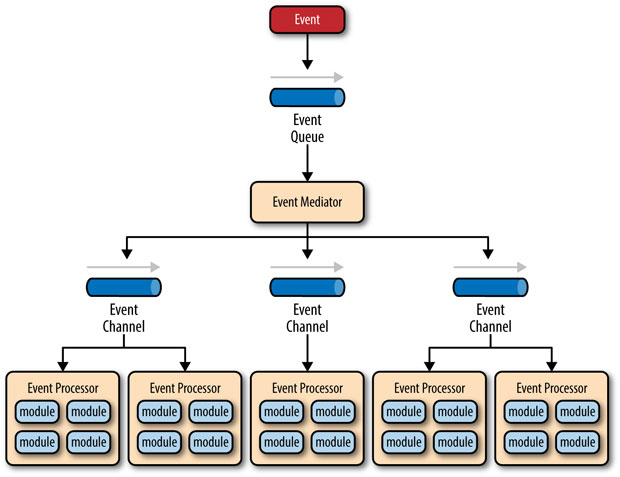
\includegraphics[width=0.9\columnwidth]{med-topology.jpg} 
    \caption{Schema Mediator Topology}
    \label{fig:eventdriver-med-top} 
\end{figure}

\paragraph{Mediatore di eventi}
Il mediatore (l’Event Mediator) ha il compito di orchestrare i passi necessari per rispondere ad un evento iniziale; per ogni passo invia uno specifico evento di processamento ad un canale (Event Channel). Il mediatore non applica nessun tipo di logica, conosce solo i passi necessari per gestire l’evento iniziale e quindi li genera.
\paragraph{Canale di eventi}
Si tratta generalmente di un canale di comunicazione asincrono. Questo può essere di due tipi:
\begin{itemize}
    \item coda di messaggi;
    \item topic di messaggi.
\end{itemize}
\paragraph{Esecutore di eventi}
Contiene la vera logica di business per processo ogni evento. Sono auto contenuti, indipendenti ed scarsamente accoppiati.



\subsubsection{Broker topology}
In questo approccio non è presente un mediatore centrale. Il flusso dei messaggi viene distribuito dai vari esecutori, creando una catena di eventi che generano a loro volta altri eventi. Risulta molto utile nel caso in cui il flusso sia molto semplice. 

In questo approccio ci sono due principali componenti:
\begin{itemize}
    \item un broker che contiene tutti i canali;
    \item vari esecutori di eventi.
\end{itemize}
    
In figura \ref{fig:eventdriven-bro-top} si riporta una generica architettura Event Driven Broker Topology.

\begin{figure}[htbp]
    \centering
    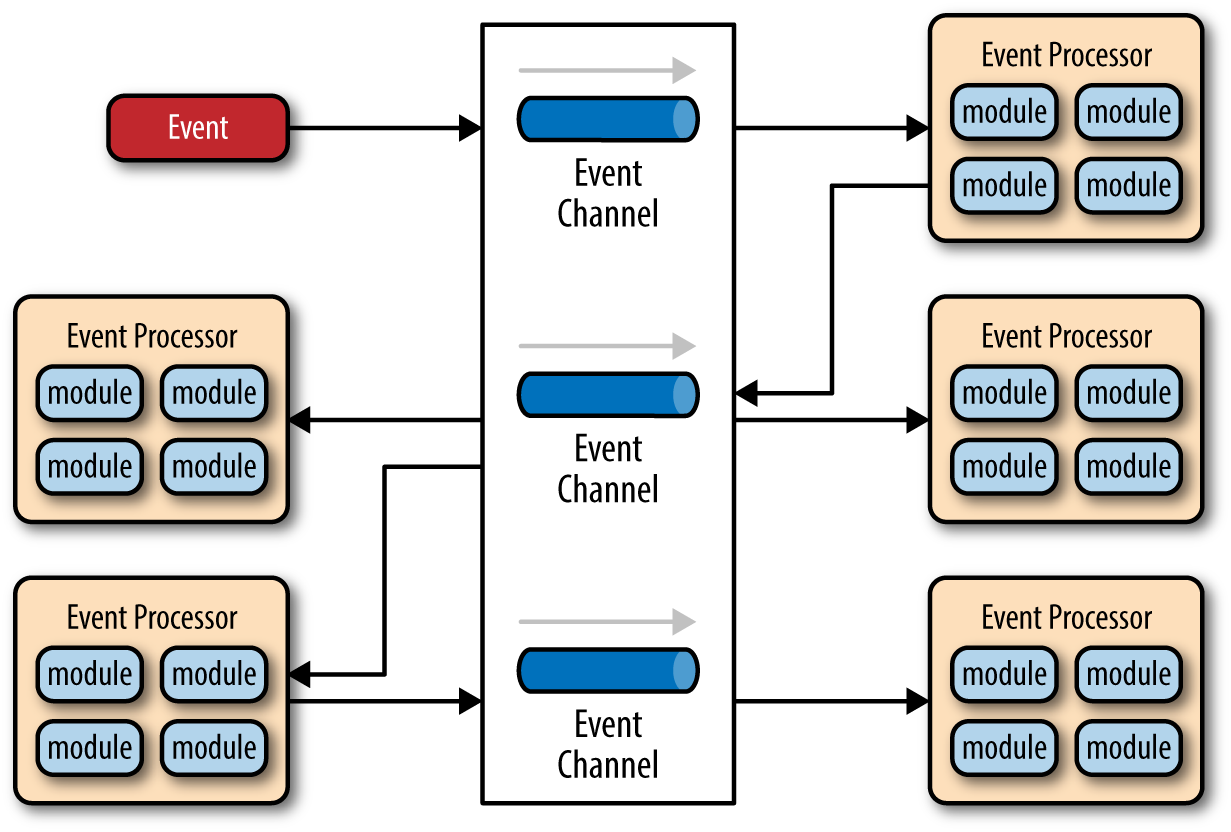
\includegraphics[width=0.9\columnwidth]{brok-top.png} 
    \caption{Schema Broker Topology}
    \label{fig:eventdriven-bro-top} 
\end{figure}

\subsubsection{Considerazioni}
Di seguito si evidenziano alcune vantaggi e svantaggi in maniera analitica \footnote{site:event-driven}:
\paragraph{Agilità generale}
I cambiamenti sono generalmente isolati e possono essere fatti velocemente con piccoli impatti.
\paragraph{Facilità di deploy}
È dovuta all’alto disaccoppiamento degli esecutori. Questa nota vale particolarmente per la tipologia Broker in quanto non presenta il mediatore.
\paragraph{Testabilità}
Richiede strumenti specializzati per generare eventi, questo potrebbe rendere i test di sistema difficoltosi. I test di unità invece sono facilmente implementabili. 
\paragraph{Scalabilità}
La natura indipendente dei componenti rende facile scalare questi in base alle necessità permettendo così un tuning delle risorse molto fine.
\paragraph{Facilità di sviluppo }
È il principale svantaggio di queste architettura.


Uno dei principali svantaggi di questo tipo di architettura è la complessità di implementazione, dovuta al fatto che operazioni sono completamente asincrone e concorrenti. Si è comunque ritenuta questa architettura nella sua variante Broker Topology adatta allo scopo soprattutto per questioni di performance, scalabilità e facilità di deploy.

\subsection{Overview}
Come già detto l’applicazione sarà strutturata con una architettura Event Driven di tipo Broker topology, questo implica che la logica di funzionamento sia incapsulata nei vari passaggi tra le varie code.
Gli esecutori sono i seguenti cinque:
\begin{itemize}
    \item \textbf{Starter}: con il compito di ascoltare gli eventi iniziali dei vari RSP e di ricevere i vari dati ottenuti tramite codici QR;
    \item RetriveInfo: con il compito di ottenere le informazioni necessarie da Monokee;
    \item \textbf{PageResponce}: con il compito di generare e visualizzare le pagine nel broswer dell’utente, sia di fallimento che di comunicazione;
    \item \textbf{PiiDataHandler}: con il compito di verificare i dati nell’ITF e verificare che questi siano sufficienti per effettuare l’accesso;
    \item \textbf{RSPSendingWork}: con il compito di inviare al RSP le informazioni di accesso.
\end{itemize}
    
Gli eventi sono i seguenti:
\begin{itemize}
    \item \textbf{AccessRequest}: generato dallo starter e eseguito dal RetriveInfo;
    \item \textbf{PageResponce}: generato dal RetriveInfo in caso di errore o per mostrare il lettore QR, dal PiiDataHandler in caso di login o in caso di insuccesso della verifica;
    \item \textbf{VerificationWork}: generato dallo Starter per verificare i dati forniti tramite il QR e quelli forniti da RequireInfo siano conformi e verificati; 
    \item \textbf{RSPSendingWork}: generato da PiiDataHandler in caso di verifica positiva.
\end{itemize}
    
 Il diagramma in figura \ref{fig:eventdriven-flusso-code} rappresenta come i vari eventi di lavoro si distribuiscono tra i vari esecutori.

 \begin{figure}[htbp]
    \centering
    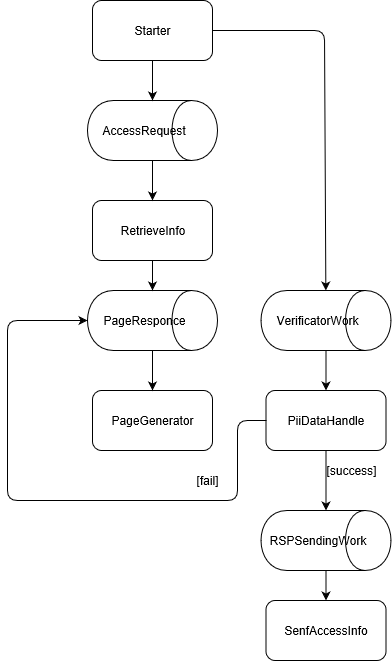
\includegraphics[width=0.9\columnwidth]{flow-eventi-sp.png} 
    \caption{Flusso eventi SP}
    \label{fig:eventdriven-flusso-code} 
\end{figure}
Lo \emph{Starter} quando riceve una richiesta d’accesso da parte del RSP procede a generare il lavoro di \emph{AccessRequest}, una volta ricavati tutti i dati necessari per l’accesso da Monokee, viene affidato al \emph{PageResponce} l’incarico di visualizzare la pagina che richiede l’inserimento del QR. I dati verranno poi inseriti dall’utente e attraverso lo \emph{Starter} verrà creato un lavoro di verifica dei dati inseriti e se questi sono sufficienti ad accedere al servizio, tramite un’ulteriore accesso a Monokee. In caso di esito positivo viene creato un lavoro di invio dati verso il RSP altrimenti verrà visualizzata una pagina di errore.
%**************************************************************
\subsection{Ciclo di vita del software}
\label{sec:ciclo-vita-software}

%**************************************************************
\subsection{Progettazione}
\label{sec:progettazione}
In figura \ref{fig:sp-uml-diag} si presenta un diagramma delle classi che attua la gestione delle code sopra espletata. Il diagramma è stato redatto in formato \emph{UML 2.0}, con leggere modifiche relativo alla rappresentazione delle varie istanze del template \emph{CommandQueue}. Questo è stato fatto al fine di rendere più leggibile e comprensibile il diagramma. Come si può notare sono presenti componenti non presenti nella precedente trattazione. Questi servono per effettuare le comunicazioni con l’ambiente esterno. Si è deciso per questioni di semplicità di non creare code separate.

\begin{figure}[htbp]
    \centering
    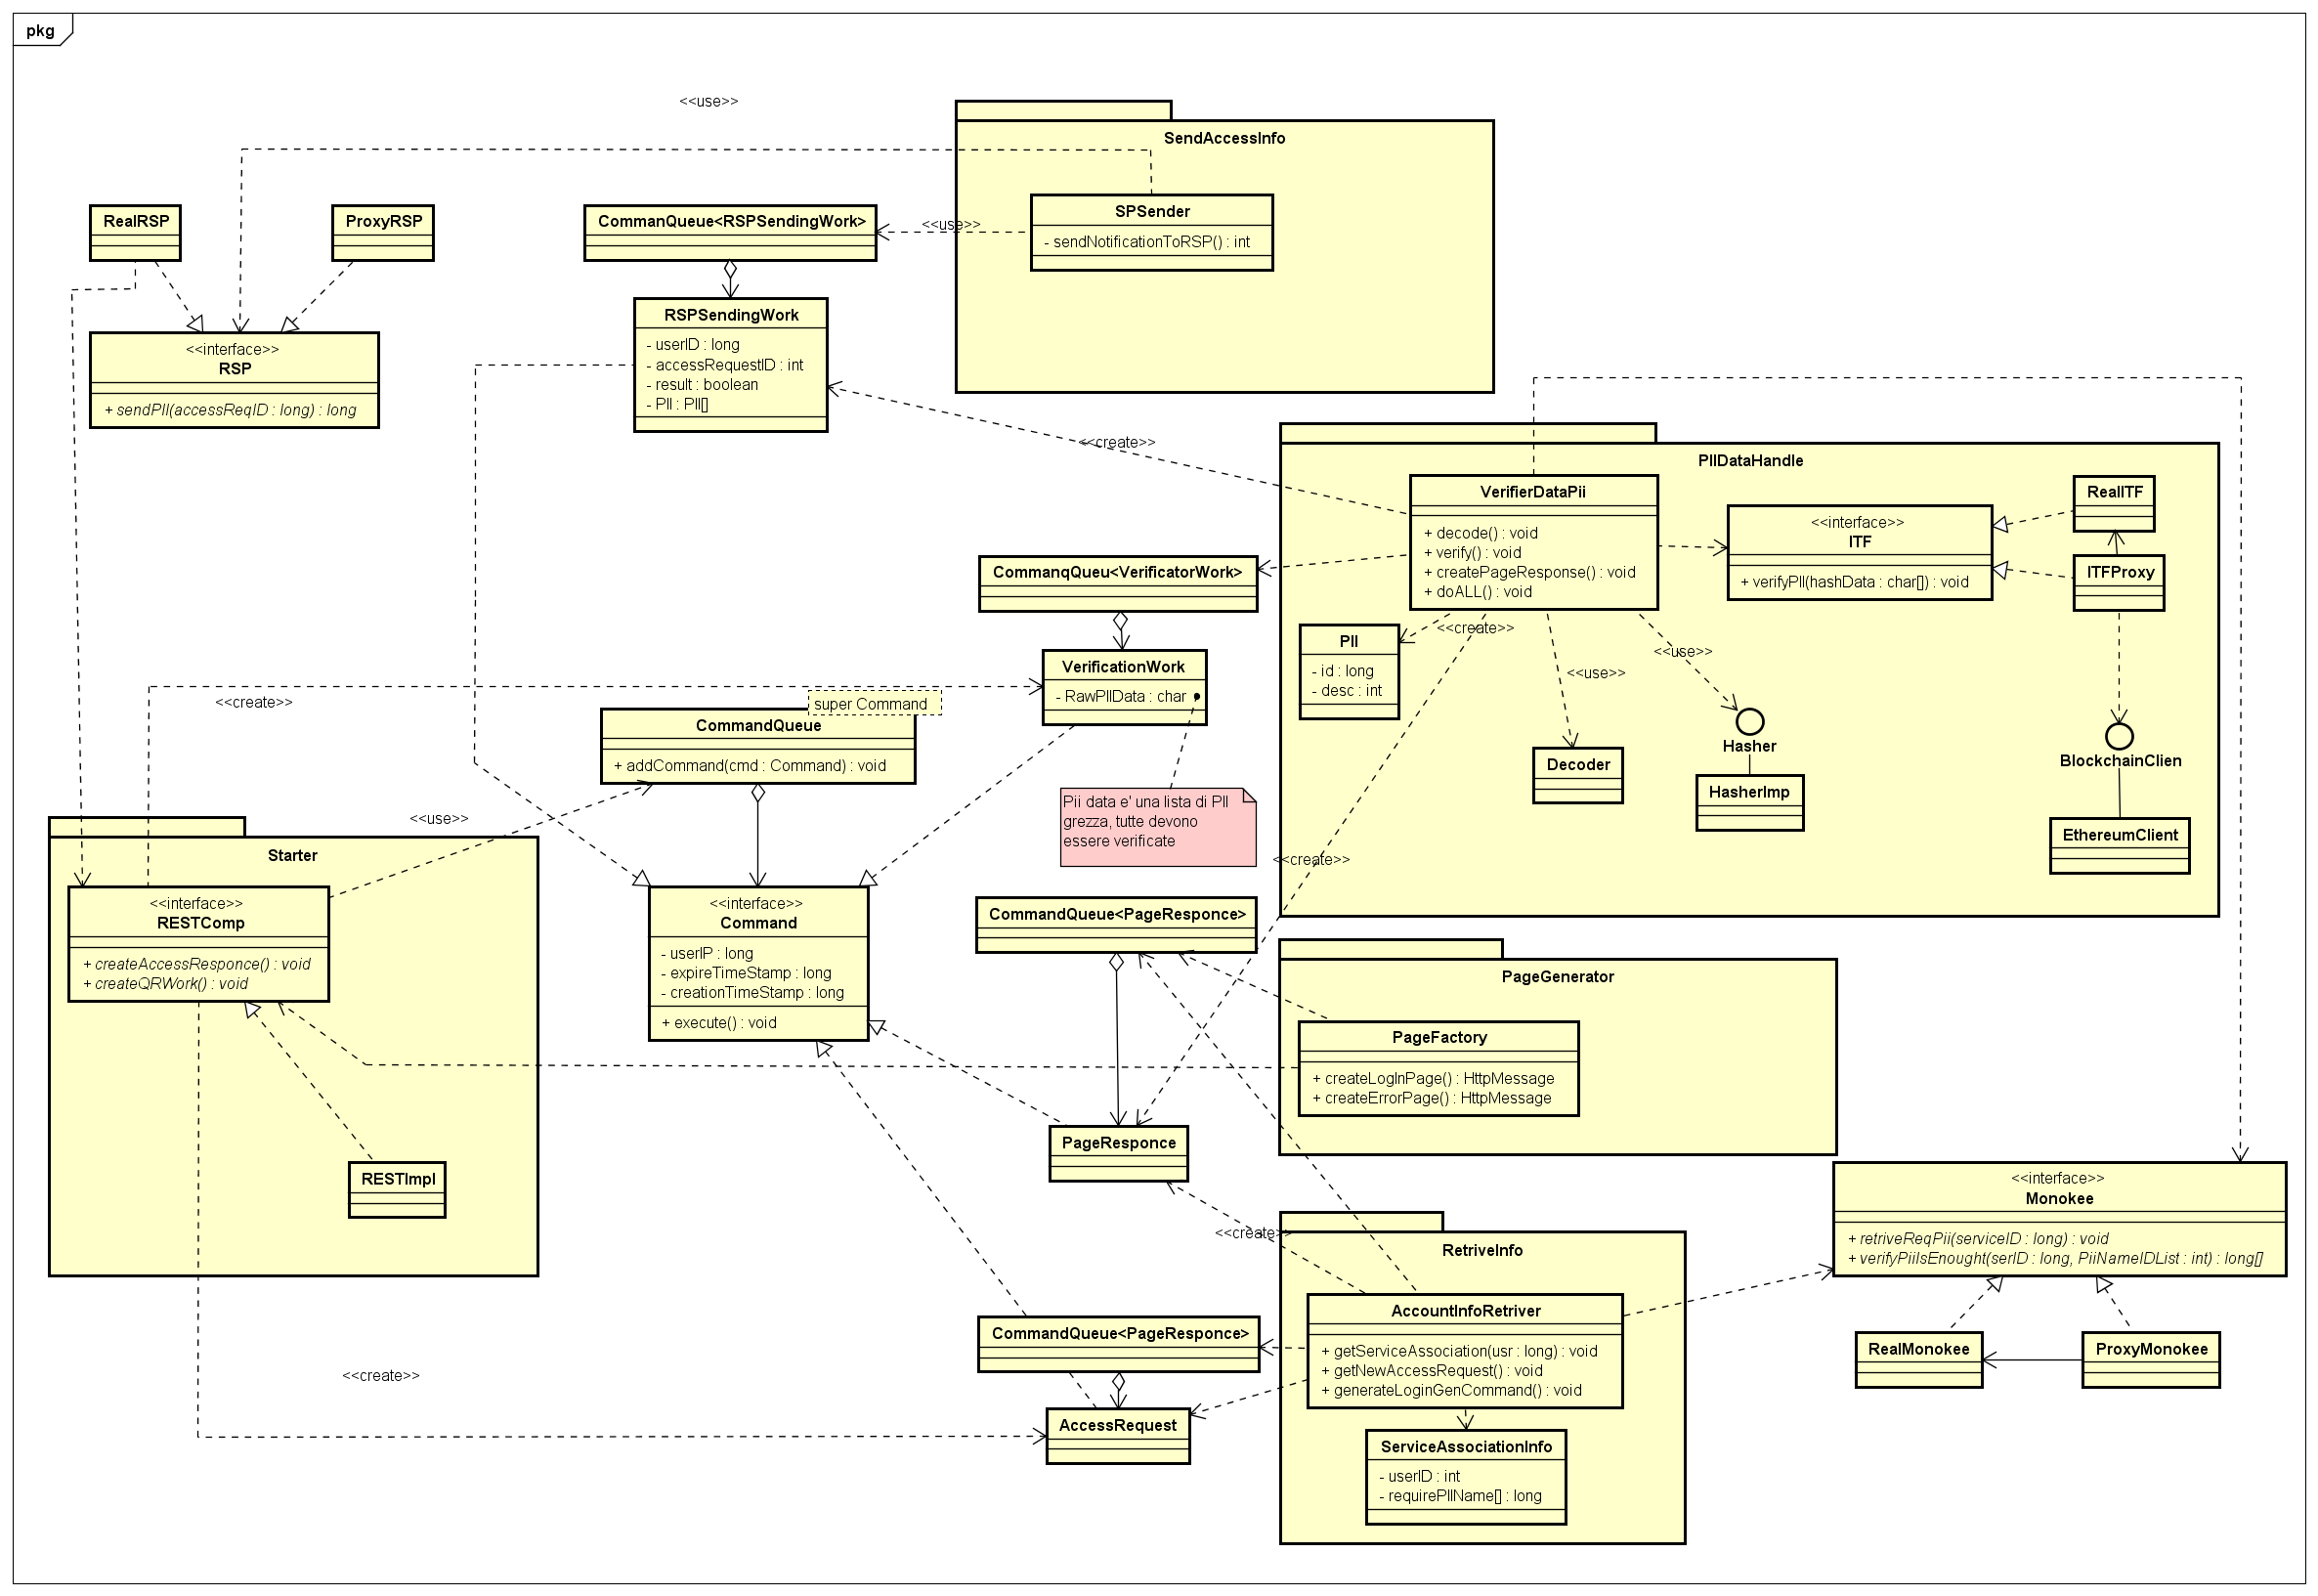
\includegraphics[width=0.9\columnwidth]{SPdiagram.png} 
    \caption{diagramma classi SP}
    \label{fig:sp-uml-diag} 
\end{figure}

\paragraph{Descrizione elementi} %**************************

\begin{namespacedesc}
    \classdesc{RESTComp}{è un’interfaccia che ha il compito di rappresentare una generica strategia di comunicazione REST. Questa viene utilizzata da RealMonokee per ottenere i dati relativi all’utente.}

    \classdesc{RESTImpl}{è una possibile implementazione della strategia di comunicazione REST. Implementa l’interfaccia RestComp.}
    \classdesc{RSP}{si tratta di un’interfaccia con il compito di fornire un’astrazione del componente real service provider. Questa interfaccia con RSPReal e ProxyRSP rappresenta un’applicazione del pattern Proxy.}
    \classdesc{RealRSP}{è una classe che rappresenta il reale oggetto RSP, questa classe poi dialoga con il RESTComp per ottenere i dati. Questa classe con RealRSP e ProxyRSP rappresenta un’applicazione del pattern Proxy.}
    \classdesc{ProxyRSP}{è una classe che rappresenta un proxy dell’oggetto RSP, questa classe applica una politica di acquisizione remota. Questa classe con RealRSP e ProxyRSP rappresenta un’applicazione del pattern Proxy.}
    \classdesc{Command}{È una classe che rappresenta un generico evento nel contesto dell’architettura event driven. Questa interfaccia viene poi implementata da:
    \begin{itemize}
        \item \textbf{AccessRequest}: generato dallo starter e eseguito dal RetriveInfo, rappresenta il lavoro per gestire la richiesta di accesso;
        \item \textbf{PageResponce}: generato dal RetriveInfo in caso di errore o per mostrare il lettore QR, dal PiiDataHandler in caso di login o in caso di insuccesso della verifica. Rappresenta il lavoro di generazione e sottomissione delle pagine all’utente;
        \item \textbf{VerificationWork}: generato dallo Starter per verificare i dati forniti tramite il QR e quelli forniti da Monokee siano conformi e verificati; 
        \item \textbf{RSPSendingWork}: generato da PiiDataHandler in caso di verifica positiva. Rappresenta il lavoro di sottomissione dati in caso di verifica positiva.
    \end{itemize}
    }
    
    \classdesc{CommandQueue}{Questo template definisce una coda di command. Dispone delle funzionalità per gestire la coda in maniera concorrente.}

    \classdesc{Account Retriver}{È la classe che ha il compito di guidare l’esecuzione di un AccessRequest. }

    \classdesc{ServiceAssociationInfo}{È una classe generata da Monokee che rappresenta un l’associazione tra utente e servizio e il nome dei PII richiesti.}

    \classdesc{Monokee}{si tratta di un’interfaccia con il compito di fornire un’astrazione del servizio Monokee. Questa interfaccia con RealMonokee e ProxyMonokee rappresenta un’applicazione del pattern Proxy.}

    \classdesc{RealMonokee}{è una classe che rappresenta il reale oggetto Monokee, questa classe poi dialoga con RESTComp per ottenere i dati. Questa classe con RealMonokee e ProxyMonokee rappresenta un’applicazione del pattern Proxy.}

    \classdesc{ProxyMonokee}{è una classe che rappresenta un proxy dell’oggetto Monokee, questa classe applica una politica di acquisizione pigra. Questa classe con RealMonokee e ProxyMonokee rappresenta un’applicazione del pattern Proxy}

    \classdesc{PageFactory}{È la classe che si occupa di eseguire l’evento PageResponce e quindi di generare le pagine e inviarle.}

    \classdesc{ITF}{si tratta di un’interfaccia con il compito di fornire un’astrazione del componente ITF. Questa interfaccia con RealITF e ProxyITF rappresenta un’applicazione del pattern Proxy.}

    \classdesc{RealITF}{è una classe che rappresenta il reale oggetto ITF, questa classe poi dialoga con il BlockchainClient per ottenere i dati. Questa classe con RealITF e ProxyITF rappresenta un’applicazione del pattern Proxy.}

    \classdesc{ITFProxy}{è una classe che rappresenta un proxy dell’oggetto ITF, questa classe applica una politica di acquisizione remota. Questa classe con RealITF e ITFProxy rappresenta un’applicazione del pattern Proxy.}

    \classdesc{VerifierDataPii}{È la classe che ha il compito di gestire i VerificationWork, si tratta di un’applicazione di Templete Patter. Ha il compito di verificare le informazioni nell’ITF e di inviare una RSPSendingWork in caso di successo o una PageResponce in caso di fallimento.}

    \classdesc{PII}{È una classe che rappresenta una PII. Contiene l’id, la descrizione di una PII.}

    \classdesc{Decoder}{è una classe che ha il compito di decodificare le informazioni presentate tramite il codice QR e quindi generare una serie di PII.}

    \classdesc{Hasher}{È un’interfaccia che ha il compito di eseguire l’hash di un dato. Rappresenta un’applicazione dello strategy pattern. }

    \classdesc{HasherImpl}{È una classe che implementa un’implementazione della classe Hasher. Esegue l’hash di un dato. Rappresenta con Hasher un’applicazione dello strategy pattern.}

    \classdesc{SPSender}{È la classe che ha il compito di eseguire i RSPSendingWork. Invia tramite il componente RestCompOut le informazioni relative l’accesso al RSP.}

\end{namespacedesc}


%**************************************************************
\subsection{Design Pattern utilizzati}
Al fine di garantire elevate doti di qualità e manutenibilità dell’architettura sono stati usati una serie di design pattern. Di seguito segue una breve descrizione di questi.


\paragraph{Command Pattern} permette di isolare la porzione di codice che effettua un'azione (eventualmente molto complessa) dal codice che ne richiede l'esecuzione; l'azione è incapsulata nell'oggetto Command. 
\paragraph{Remote Proxy} fornisce una rappresentazione locale di un oggetto remoto remote. 
\paragraph{Strategy Pattern} è un oggetto che permette di separare l’esecuzione di un metodo dalla classe che lo contiene. Usando un’interfaccia per astrarre il metodo è poi possibile crearne molteplici implementazioni. Questo è risultato molto utile nel contesto di un’applicazione multi piattaforma in cui alcune procedure andavano implementate in nativo. Oltre all’appena citato vantaggio questo ha reso possibile separare il metodo dall’implementazione. 
\paragraph{Dependency Injection} è un pattern che permette di delegare il controllo della creazione oggetti ad un oggetto esterno. Questo permette di semplificare la gestione delle dipendenze e nel contesto dello strategy pattern permette di inoculare l’implementazione corretta. 
\paragraph{Factory Method} è un pattern che permette di convogliare tutte le funzioni di creazione di vari elementi ad un oggetto unico. 

%**************************************************************
\section{Implementazione}

Le attività di implementazione e codifica sono state la parte di maggior impegno e sforzo dell'intero progetto. Hanno occupato in termini orari 120 ore, le quali rappresentano quasi il 40\% della durata del progetto. Esse hanno fatto emergere diversi errori di progettazione e di codifica, inoltre ci sono stati diverse ripensamenti da parte dell'azienda che hanno portato a riprogettare interi moduli. Nei paragrafi seguenti si cercherà di presentare le implementazioni più significative all'interno del progetto.

\subsection{Procedura di login}
L'applicativo mobile non prevedeva una gestione degli account propria, ma utilizzava gli account già presenti nel sistema Monokee. Questo ha necessitato quindi la codifica di un apposita procedura di login in modo di autenticare un utente in base ad una coppia di valori email e password. 

La suddetta procedura consiste principalmente in due chiamate HTTPS, la prima con lo scopo di ottenere l'id dell'utente tramite la mail fornita, la seconda allo scopo di verificare se la password sia conforne all'id ottenuto dalla prima chiamata. 

La prima fase era attuata da un metodo chiamato \textbf{Task<string> RetriveUserID(string usr)}. Questo metodo inviava tramite una POST il seguente json, con il quale forniva le informazioni necessarie ad ottenere l'id :

\begin{lstlisting}[caption={Json della prima request di login}]
    {
        email = "user@dominio.com",
        mobile = "false",
    }
\end{lstlisting}

La risposta doveva invece seguire il seguente schema:

\begin{lstlisting}[caption={Json risposta user\_id}]
    {
        success = "true",
        message = "ok",
        user_id = "df3c92kzz1",
    }
\end{lstlisting}

La risposta in alcuni casi poteva presentare altri campi dati, ma questi venivano ignorati dall'applicativo. Risposte che non presentavano le precedentemente citate tre informazione o che non riportavano i valori "true" ed "ok" rispettivamente su "success" e "message" causavano il lancio di un'eccezzione che faceva comparire un messaggio di fallimento a schermo.

Una volta ottenuto il valore "user\_id" si procedeva alla verifica della password col metodo
\textbf{getTokenID(string userId, string password)}.
Questo avveniva sempre tramite l'uso di una comunicazione POST. Nella request veniva mandato il seguente json:

\begin{lstlisting}[caption={Json richiesta token}]
    {
        user_id = "df3c92kzz1",
        password = "Passw0rd",
        mobile = "false",
        persistence = "false",
        cc_key = "key",
        salt = "salt",
        domain_id = "5b475bd150e783334b5bb861",
    }
\end{lstlisting}

Il campo "persistence" è utile alla gestione interna del dato e non rientra in nessun modo nel progetto.
I parametri "cc\_keys" e "salt" invece sono due valori tipici delle procedure di login. Questi servono a rendere più complessi gli attacchi a dizionario verso il sistema, infatti i due valori per essere generati richiedono un elevato onere computazionale sia in termini di spazio che di tempo, in quanto devono rispettare delle determinate condizioni. La codifica del codice per generare questi due valori ha richiesto innumerevoli sforzi e si è rivelata essere non banale.
L'applicativo Monokee ha la caratteristica di offrire ai propri utenti domini seperati, un tipico utilizzo di questi è per esempio il dominio aziendale e quello personale. Il "domain\_id" fornito da rappresenta il dominio personale. L'applicativo per ragioni di semplicità faceva l'accesso sempre allo stesso dominio. 

La risposta doveva seguire il seguente schema:
\begin{lstlisting}[caption={Json risposta token}]
    {
        success = "true",
        message = "ok",
        token = "qrdj99d7f9da0b2nf93Kd9LL"
    }
\end{lstlisting}

Il significato di "success" e "message" rimane analogo a quello precedentemente descritto, mentre il valore "token" rappresenta un codice da inserire nell'header sotto il nome di "Authorization" nelle successive chiamata in modo tale da essere risposto. Questo codice ha validità di 24 ore, al seguito delle quali scade ed è necessario rieffettuare la procedura di login. Risulta estremamente importante al momento del logout rimuovere dall'header il token, in quando una successiva operazione di login ne avrebbe aggiunto un altro causando un doppio token. Questo avrebbe fatto fallire le successive richiesta, seppur consentendo l'accesso.

Per ragioni progettuali interne a Monokee le chiamate se ricevute vengono sempre risposte con uno status code 200, a prescindere del fatto che queste siano accettate o rifiutate. Per questa ragione al fine di sostituire i vari codici di errore vengono usati i campi "success" e "message". 

La codifica di questa procedura non ha presentato particolari difficolta se non quella della generazione del cc\_key e del salt. 

\subsection{Uso del database SQLite}

Nel contesto dell'applicazione mobile per effettuare la persistenza dei dati si è deciso di utilizzare una base di dati relazionale. La scelta è ricaduta su SQLite. Si è deciso di operare con questa base di dati utilizzando il design pattern \emph{data access object} e apposite libreria di sistema che lo implementavano, questa pratica si è rivelata essere molto pratica ed efficace ai fini del progetto. Ovviamente risulta limitata comparata rispetto all'uso del codice \emph{sql}, ma le necessità applicative non richiedevano simili finezze.

A titolo di esempio si discute ora della memorizzazione di un PII.

\begin{lstlisting}[caption={codice creazione DAO}]
    public DBDao()
    {
        database = DependencyService
            .Get<ILocalDataProvider>()
            .GetConnection();
        database.CreateTable<PIIModel>();
        database.CreateTable<UserModel>();
    }
\end{lstlisting}

Il codice appena presentato rappresenta la creazione dell'oggetto che fornisce l'accesso alla base di dati, come si può notare il corpo del costrutture crea una connessione tramite l'uso di \emph{DependencyService}, successivamente crea le tabelle. Ovviamente in caso le tabelle siano già presenti, le istruzioni non alterano la base di dati. 

A differenza di quanto uno si potrebbe aspettare, la funzione \emph{CreateTable} non richiede informazione sui tipi di dato e/o sulle colonne da creare. Queste informazione vengono dedotte dal tipo che gli viene fornito, il quale andrà a rappresentare il modello di una tupla della tabella.

Si propone adesso il codice di \emph{PIIModel}:
\begin{lstlisting}[caption={codice PIIModel}]
    [Table("PIIModel")]
    public class PIIModel
    {
 
        [PrimaryKey, AutoIncrement]
        public int Id;
        
        [Indexed(Name = "nameId", Order = 1, Unique = true)]
        public string UserID;

        [Indexed(Name = "nameId", Order = 2, Unique = true)]
        public string Name;
        [NotNull]

        //continua ...
\end{lstlisting}

I campi dati pubblici vengono considerati come i valori delle colonne, mentre altre informazioni necessarie vengono fornite tra parentesi quadre. Queste sono per esempio le chiavi, i valori non nulli, i vincoli di integrità, il nome della tabella etc...

Sequendo questa tecnica la gestione del database risulta particolarmente semplice. Vengono ora riportati degli esempi di codice per l'inserimento e la rimozione di una PII dalla base di dati:

\begin{lstlisting}[caption={codice aggiunta e rimozione PIIModel}]
public int AddPII(PIIModel pii)
    {
        lock (collisionLock)
        {
            if (pii.Id != 0)
            {
                database.Update(pii);
                return pii.Id;
            }
            else return database.Insert(pii);      
        }
    }

public int DeletePII(int piiID)
{
    lock(collisionLock)
    {
        return database.Delete<PIIModel>(piiID);
    }
}
\end{lstlisting}

Ovviamente query più complicate risultano non essere possibile tramite funzioni di libreria, per queste particolari occassioni si è dovuto utilizzare del codice sql.

\begin{lstlisting}[caption={Esempio di query sql}]
public List<PIIModel> GetPIIs(string name, string user\_id)
    {
        lock (collisionLock)
        {
            return (from i in database.Table<PIIModel>()
                    where (i.Name == name && i.UserID==user\_id)
                    select i).ToList();
        }
    }
\end{lstlisting}

L'uso di queste tecniche e dei modelli ha permesso di limitare al massimo l'utilizzo di codice sql, inoltre ha permesso una più facile gestione del dato in quanto la risposta ad una query veniva già presentata in forma di oggetto.

\subsection{Implementazione del databinding}
L'applicaione mobile richiedeva la creazione di molteplici schermate che dovevano sempre rimanenere aggiornare rispetto ad un particolare oggetto e viceversa. Questo risultava particolarmente importante in quanto era fondamentale che l’interfaccia fosse ben separata dalla logica di business, affinché una modifica nella logica o nel modello di dominio non si rifletta sull’interfaccia. 

A questi scopi \emph{Xamarin} offre la cosidetta tecnica del databinding tra intefaccia e oggetto. Ora si ripropone l'oggetto PIIModel, questa volta però non omettendo il codice necessario per il databinding.

\begin{lstlisting}[caption={esempio di oggetto in databinding}]
[Table("PIIModel")]
public class PIIModel : INotifyPropertyChanged
{
    private int piiID;
    [PrimaryKey, AutoIncrement]
    public int Id
    {
        get { return piiID; }
        set {
            piiID = value;
            OnPropertyChanged(nameof(Id));
        }
    }

    \\altro codice ommesso ...

    private void OnPropertyChanged(string propertyName)
    {
            PropertyChanged?.Invoke(this,
            new PropertyChangedEventArgs(propertyName));
    }
}
\end{lstlisting}

Come si può notare per poter effettuare il databinding è necessario che la classe PIIModel implementi l’interfaccia INotifyPropertyChanged, che definisce l’evento PropertyChanged di tipo PropertyChangedEventHandler. Questo evento prende un’istanza della classe PropertyChangedEventArgs che definisce la proprietà PropertyName di tipo string, attraverso la quale è possibile sapere quale proprietà nell'oggetto PIIModel è cambiata (permettendo all’evento di accedere a quella proprietà).

Attraverso la proprietà pubblica Id, offriamo la possibilità lato codice di ottenere le informazioni sul valore corrente attraverso il get, e di impostare un nuovo valore per tale proprietà attraverso il set ogni qualvolta il valore assunto dalla variabile name differisce da quella corrente. Proprio in quest’ultima porzione viene richiamato il metodo OnPropertyChanged, che prenderà in ingresso il nome della proprietà che deve essere aggiornata innescando il meccanismo sopra descritto. 

Per effettuare l'effettiva collegamento basta inserire nel codice che gestische la schermata la seguente istruzione:
\begin{lstlisting}[caption={codice di connessione}]
    BindingContext = PIIModel;
\end{lstlisting}

Questo renderà possibile nel codice grafico (XAML) di poter utilizzare i valori dell'oggetto. Di seguito viene mostrato un esempio:

\begin{lstlisting}[caption={esempio di vista che usa il databinding}]
<?xml version="1.0" encoding="utf-8" ?>
<ContentPage xmlns="http://xamarin.com/schemas/2014/forms"
             xmlns:x="http://schemas.microsoft.com/winfx/2009/xaml"
             x:Class="IdentityWallet.PIIVisualizerPage"
             Title="{Binding Name}">
    <ContentPage.Content>
        <ScrollView>
            <StackLayout VerticalOptions="StartAndExpand" Padding="20">
                <Label Text="Id"/>
                <Label x:Name="piiID" Text="{Binding Id}"/>
            
                <Label Text="Name" />
                <Entry x:Name="piiName" Text="{Binding Name}"/>
            
                <- altro codice ->
            </StackLayout>
        </ScrollView>
    </ContentPage.Content>
</ContentPage>
\end{lstlisting}

\subsection{Instaurazione della rete di messaggi}
Il modulo SP è composto da diversi componenti, i quali sono residenti in programmi differenti e seperati fra loro. L'unico modo di comunicazione che utilizzano è un \gls{messagebrokerg}\glsfirstoccur di nome \emph{RabbitMQ}. Questo deve essere eseguito su un server e verrà utilizzato dai vari componenti tramite il suo \emph{uri}.
L'applicativo richiede che nel server sia installato \emph{Erlang}. Una volta averlo installato si può procedere all'installazione di \emph{RabbitMQ} seguendo la guida presente al seguente url \url{https://www.rabbitmq.com/download.html}. Per eseguire correttamente le funzionalità del modulo SP è inoltre necessario creare una rete col nome di "test"; per fare questo è necessario abilitare l'interfaccia di configurazione di \emph{RabbitMQ} seguendo la seguente guida \url{https://www.rabbitmq.com/management.html}.
Una volta abilitata l'interfaccia questa sarà disponibile al seguente indirizzo \url{http://localhost:15672/#/connections}. La pagina che si presenterà avrà una scheda chiamata "network" dalla quale sarà possibile aggiungere la rete di nome "test".
Fatto questa la configurazione di \emph{RabbitMQ} è terminata; ora basta avviare il broker tramite terminale usando il comando \emph{rabbitmq-server start}.


\subsection{Gestione delle code e dei messaggi}
Come già discusso il modulo SP ha un'architettura del tipo \emph{even driven}. L'applicazione di tale libreria ha necessitato dell'uso di una libreria per la gestione e l'invio dei vari messaggi.

Il modulo SP è diviso in molteplici esecutori ognuno del quale presente del codice per la gestione dei messaggi equivalente, a titolo di esempio si procede ad esporre l'esecutore \emph{ITFVerifier}.

All'avvio l'esecutore ha il compito di creare un oggetto in grado di individuare la rete che gestisce i messaggi (questa era disponibile all'uri definito in \emph{GeneralSetting.RabbitMQHost}) e quindi effettuare il collegamento ad essa tramite la sottomissione di una coppia username, password.
Successivamente era necessario definire cosa doveva essere fatto dei messaggi in arrivo e sopratutto quale tipo di messaggi dovessero essere ascoltati. La parte finale del codice propostro mostra le instruzione necessarie a fare quanto appena detto. Tramite \emph{ReceiveEndpoint} viene stabilito il nome della coda dove verranno inseriti i messaggi catturati e il comportamento da intraprendere per ognuno di questi messaggi. Come comportarsi viene definito tramite una arrow function che instanzia un \emph{Consumer} con un tipo da noi definito (\emph{VerificationWorkConsumer}). I messaggi da inserire nella code di ricezione non vengono decisi in base ad un'indicazione del mandante, ma tramite il tipo dell'oggetto che implementa \emph{VerificationWorkConsumer}.
L'ultimi riga ha lo scopo di eseguire il lavoro in modalità asincrona.
\begin{lstlisting}[caption={creazione di un collegamento a \emph{RabbitMQ}}]
    _busControl = Bus.Factory.CreateUsingRabbitMq(x =>
        {
            IRabbitMqHost host = x.Host(new Uri(GeneralSetting.RabbitMQHost), h =>
            {
                h.Username("guest");
                h.Password("guest");
            });
            
            x.ReceiveEndpoint(host, "VerQueue",
                e => { e.Consumer<VerificationWorkConsumer>(); });
            
        });

        TaskUtil.Await(() => _busControl.StartAsync());
\end{lstlisting}

Adesso risulta utile analizzare il codice del \emph{Consumer}. Come si può notare la classe implementa \emph{IVerificationWork}, pertando nella coda che porta il nome di "VerQueue" verranno inseriti solo i messaggi che hanno come tipo \emph{IVerificationWork}.
Unico metodo implementabile è \emph{Consume} il quale rappresenta il codice da effettuare.

\begin{lstlisting}[caption={esempio di \emph{Consumer}}]
public class VerificationWorkConsumer : IConsumer<IVerificationWork>
{
    public async Task Consume(ConsumeContext<IVerificationWork> context)
    {
            //operazioni da effettuare

    }
}
\end{lstlisting}

Andiamo ora a vedere come si invia un messaggio un \emph{VerificationWork}:
\begin{lstlisting}[caption={codice invio di un messaggio}]
    public async Task SendToVerificationAsync(IVerificationWork verWork)
    {
        await _busControl.Publish(verWork);
    }
\end{lstlisting}

Come potete vedere questo avviene tramite la funzione \emph{Publish} dell'oggetto \emph{\_busControl}.

\subsection{Interazioni con la \emph{blockchain}}

Sia l'applicativo mobile IW, che l'applicativo server SP hanno previsto l'uso della stessa libreria \emph{Nethereum} al fine di effettuare le necessarie chiamate alla \emph{blockchain Ethereum}.
Questa libreria implementa il protocollo Ethereum\footcite{site:ethereum-yellow-paper} in ambiente \emph{.NET}.

Il protocollo discerne tra due tipi di chiamate, quelle in \textbf{sola lettura} e quella \textbf{in scrittura}; le prime sono identificate dai modificatori \emph{pure} o \emph{view}.

Le chiamate in sola lettura sono immediate e non richiedono l'esecuzione di una transazione, per queste ragioni hanno prestazione paragonabile a quelle di un linguaggio tradizionale e non richiedono le venga fornito dell'\gls{etherg}.

Le seconde invece, dovendo modificare la blockchain, hanno bisogno di effettuare una transazione con la conseguente esecuzione dell'algoritmo di consenso descritto nel capitolo \ref{cap:alg-cons}. Questo porta ai problemi di prestazioni e costo descritti in \ref{cap:prestazioni}

Prima di poter procedere a qualsiasi operazione era necessario creare un collegamente alla rete \emph{Ethereum} usata (nel nostro caso una rete locale all'azienda). Il sequente codice mostra le istruzioni necessarie.

\begin{lstlisting}[caption={Connessione alla rete di test},label={lst:connessione},language={C}]
account = new Account(GeneralSetting.accountPrivKey);
web3 = new Web3(account, blockchain_address);
\end{lstlisting}

La variabile \emph{web3} è l'oggetto che rappresenta la connessione. Il primo parametro del costruttore non è strettamente necessario, ma stabilisce un account di default con il quale verranno pagate le transazioni. Si è deciso in fase di codifica di non minare direttamente le aggiunte di blocchi, ma di pagare la transazione. Per essere riconosciuti dalla rete è sufficiente fornire la chiave privata. 
\medskip

Ora è necessario richiamare un contratto presente nella rete. Per fare questo necessitiamo di due informazione: l'\textbf{indirizzo} e l'\gls{abig}\glsfirstoccur. L'\emph{ABI} di un contratto consiste in un json contenente la definizione di tutti i metodi presenti nel contratto. Nel frammento ~\ref{lst:abi_ex} si mostra l'\emph{ABI} della chiamata che andremo ad effettuare, invece nel frammento ~\ref{lst:creazioneContr} si mostra la creazione dell'oggetto contratto. Dal contratto poi si ottiene la funzione.

\begin{lstlisting}[caption={Esempio di ABI},label={lst:abi_ex},language={C}]
[
    {
        "anonymous": false,
        "inputs": [
            {
                "indexed": true,
                "name": "_PII_ID",
                "type": "string"
            },
            {
                "indexed": false,
                "name": "result",
                "type": "bool"
            }
        ],
        "name": "eventResponse",
        "type": "event"
    },
    {
        "constant": false,
        "inputs": [
            {
                "name": "_publicKey",
                "type": "string"
            },
            {
                "name": "_PII_ID",
                "type": "string"
            },
            {
                "name": "_name",
                "type": "string"
            },
            {
                "name": "_description",
                "type": "string"
            }
        ],
        "name": "verify",
        "outputs": [
            {
                "name": "",
                "type": "bool"
            }
        ],
        "payable": false,
        "stateMutability": "nonpayable",
        "type": "function"
    }
]  
\end{lstlisting}

\begin{lstlisting}[caption={Creazione del contratto},label={lst:creazioneContr},language={[Sharp]C}]
    SPFContract = web3.Eth.GetContract(abi,
                "contract_address");
    var verifyFunction = SPFContract.GetFunction("verify");
\end{lstlisting}

Una volta ottenuto l'oggetto \emph{verifyFunction} non ci resta che effettuare la chiamata. Il metodo \emph{verify} effettua modifiche, quindi è necessario effettuare una transazione. La funzione \emph{SendTransactionAndWaitForReceiptAsync} effettua la chiamata del metodo solidity \emph{verify} e aspetta che questa fallisca o abbia successo. Una transazione non restituisce mai il risultato della chiamata, ma una ricevuta che ne attesta la riuscita o il fallimento. Per ottenere il risultato bisogna usare i cosidetti \emph{eventi} che vanno lanciati dal codice solidity con il contenuto del valore di ritorno. Gli eventi sono comunicati in \emph{broadcast} a tutti gli utenti connessi alla rete, di conseguenza ottenere il risultato richiede una serie di procedure particolari. La seconda parte del codice nel frammento  \ref{lst:transax} mostra il codice necessario per filtrare gli eventi in base alla ricevuta e quindi ottenere il valore. 


\begin{lstlisting}[caption={Creazione del contratto},label={lst:transax},language={[Sharp]C}]
receipt = await verifyFunction.SendTransactionAndWaitForReceiptAsync(
    "account_address,
    null, 
    ITFID,
    description, 
    publicKeyBytes)
    .ConfigureAwait(false);          

    //CODICE PER GESTIRE L'EVENTO DI RISPOSTA
    var verifyEvent = SPFContract.GetEvent("eventResponse");
    var filterOnITFID = verifyEvent.CreateFilterInput(
        new BlockParameter(receipt.BlockNumber),
            BlockParameter.CreateLatest());
    var log = await verifyEvent.GetAllChanges<VerificationEvent>(filterOnITFID);
    result = log[0].Event.Result;
\end{lstlisting}


Le chiamate a metodi solidity detti \emph{puri}, invece, sono più semplici e restituiscono direttamente il risultato.
Di seguito un esempio di una chiamata di questo tipo.

\begin{lstlisting}[caption={Esempio di chiamata a metodo puro},label={lst:call_ex},language={[Sharp]C}]

getFunction = SPFContract.GetFunction("getFromID");
string result = await getFunction.CallAsync(par1, par2);
    
\end{lstlisting}


\subsection{Procedura di accesso a servizio}
Di seguito viene esposte le varie azione che vengono scatenate durante una tipica operazione di accesso ad un servizio. Il progetto è compatibile con tutti i servizi compatibili con lo standard \gls{samlg}.

\noindent Si propone come esempio l'applicativo \emph{Salesforce}.

Tramite l'interfaccia di \emph{Salesforce} abbiamo creato un apposito dominio di accesso. In questo modo l'utente potrà in fase di login specificare il dominio con il quale effettuare l'accesso.
Le immagini \ref{fig:salesforce-login} e \ref{fig:salesforce-dom} mostrano come indicare il dominio.

\begin{figure}[!h]
    
    \centering
    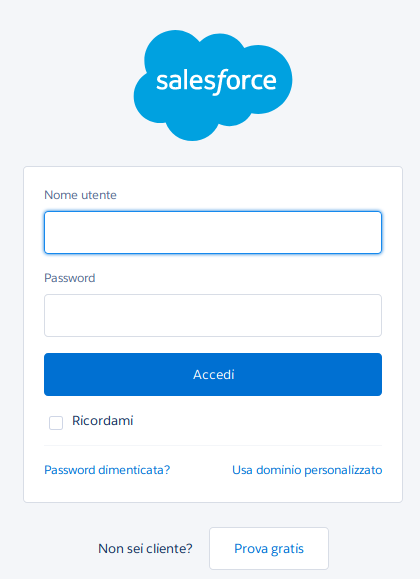
\includegraphics[width=0.4\columnwidth]{login.png} 
    \caption{Schermata di login di Salesforce}
    \label{fig:salesforce-login} 
\end{figure}

\begin{figure}[!h]
    
    \centering
    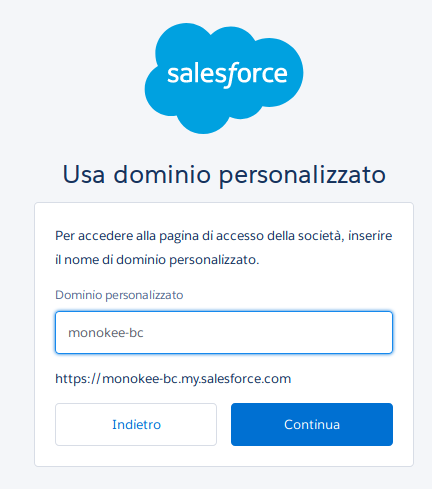
\includegraphics[width=0.4\columnwidth]{dominioLogin.png} 
    \caption{Schermata di scelta dominio}
    \label{fig:salesforce-dom} 
\end{figure}

Indicando il dominio corretto il browser procederà a reindirizzare l'utento presso un apposito sito interno al \emph{back-end} di Monokee.

L'inoltro verso il sito scatenerà le seguenti operazioni:
\begin{enumerate}
    \item collegamento verso un canale \gls{websocketg} gestito dal componente \emph{ResultSender} del modulo SP;
    \item attivazione della web-cam del computer e cattura di immagini fino all'individuazione di un codice QR compatile con quello generato dall'applicativo mobile IW;
    \item invio tramite comunicazione POST del contenuto del codice QR al modulo SP, la risposta alla POST conterrà un \gls{nonceg} da usare in seguito;
    \item verifica da parte del componente SP delle informazioni di accesso fornite tramite la POST e quindi invio del risultato e del \emph{nonce} tramite il canale \emph{WebSocket}. Il componente SP si occuperà inoltre di comunicare l'esito anche al \emph{back-end} di Monokee, il quale si occuperà della generazione della \emph{SAMLResponse}\footnote{La SAMLResponse consiste in \emph{XML} contenente tutte le informazioni necessarie a Salesforce per permettere l'accesso. Volendo fare un esempio nel caso di un servizio che richieda username e password, l'\emph{XML} conterrà questi due dati con l'aggiunta di una serie di firme e informazione utili a garantire la sicurezza del protocolo. Per maggiori dettagli consultare \url{https://www.samltool.com/generic_sso_res.php}.} corrispondente;
    \item inserimento della \emph{SAMLResponse} da parte del \emph{back-end} di Monokee all'interno di una form presente nel sito;
    \item ricezione da parte del sito dell'esito della verifica tramite il canale \gls{websocketg};
    \item verifica dell'uguaglianza del \emph{nonce} ricevuto dalla POST con quello ricevuto dall'esito della verifica e verifica della positività dell'esito ;
    \item in caso entrambe le verifiche abbiamo riscontro positivo invio tramite POST della \emph{SAMLResponse} al \emph{back-end} di Salesforce;
    \item reindirizzamento verso l'applicativo Salesforce. Ora si è riconosciuti come utenti.
\end{enumerate}

\noindent Qualora una qualsiasi delle precedenti operazioni fallisse o desse esito negativo il sito mostrerà un messaggio di errore a schermo e richiederà la risottimissione del codice QR.
